%%%%%%%%%%%%%%
%% Run LaTeX on this file several times to get Table of Contents,
%% cross-references, and citations.

%% If you have font problems, you may edit the w-bookps.sty file
%% to customize the font names to match those on your system.

%% w-bksamp.tex. Current Version: Feb 16, 2012
%%%%%%%%%%%%%%%%%%%%%%%%%%%%%%%%%%%%%%%%%%%%%%%%%%%%%%%%%%%%%%%%
%
%  Sample file for
%  Wiley Book Style, Design No.: SD 001B, 7x10
%  Wiley Book Style, Design No.: SD 004B, 6x9
%
%
%  Prepared by Amy Hendrickson, TeXnology Inc.
%  http://www.texnology.com
%%%%%%%%%%%%%%%%%%%%%%%%%%%%%%%%%%%%%%%%%%%%%%%%%%%%%%%%%%%%%%%%

%%%%%%%%%%%%%
% 7x10
%\documentclass{wileySev}

% 6x9

\documentclass{wileysix}
\UseRawInputEncoding
\usepackage{graphicx}
\usepackage{listings}

\usepackage{float}

\usepackage{color}
 
\definecolor{codegreen}{rgb}{0,0.6,0}
\definecolor{codegray}{rgb}{0.5,0.5,0.5}
\definecolor{codepurple}{rgb}{0.58,0,0.82}
\definecolor{backcolour}{rgb}{0.95,0.95,0.92}
 
\lstdefinestyle{mystyle}{
    backgroundcolor=\color{backcolour},   
    commentstyle=\color{codegreen},
    keywordstyle=\color{magenta},
    numberstyle=\tiny\color{codegray},
    stringstyle=\color{codepurple},
    basicstyle=\footnotesize,
    breakatwhitespace=false,         
    breaklines=true,                 
    captionpos=b,                    
    keepspaces=true,                 
    numbers=left,                    
    numbersep=5pt,                  
    showspaces=false,                
    showstringspaces=false,
    showtabs=false,                  
    tabsize=2,
    language=sh
}
 
\lstset{style=mystyle}

%%%%%%%
%% for times math: However, this package disables bold math (!)
%% \mathbf{x} will still work, but you will not have bold math
%% in section heads or chapter titles. If you don't use math
%% in those environments, mathptmx might be a good choice.

% \usepackage{mathptmx}

% For PostScript text
\usepackage{w-bookps}

%%%%%%%%%%%%%%%%%%%%%%%%%%%%%%%%%%%%%%%%%%%%%%%%%%%%%%%%%%%%%%%%
%% Other packages you might want to use:

% for chapter bibliography made with BibTeX
% \usepackage{chapterbib}

% for multiple indices
% \usepackage{multind}

% for answers to problems
% \usepackage{answers}

%%%%%%%%%%%%%%%%%%%%%%%%%%%%%%
%% Change options here if you want:
%%
%% How many levels of section head would you like numbered?
%% 0= no section numbers, 1= section, 2= subsection, 3= subsubsection
%%==>>
\setcounter{secnumdepth}{3}

%% How many levels of section head would you like to appear in the
%% Table of Contents?
%% 0= chapter titles, 1= section titles, 2= subsection titles, 
%% 3= subsubsection titles.
%%==>>
\setcounter{tocdepth}{2}

%% Cropmarks? good for final page makeup
%% \docropmarks

%%%%%%%%%%%%%%%%%%%%%%%%%%%%%%
%
% DRAFT
%
% Uncomment to get double spacing between lines, current date and time
% printed at bottom of page.
% \draft
% (If you want to keep tables from becoming double spaced also uncomment
% this):
% \renewcommand{\arraystretch}{0.6}
%%%%%%%%%%%%%%%%%%%%%%%%%%%%%%

%%%%%%% Demo of section head containing sample macro:
%% To get a macro to expand correctly in a section head, with upper and
%% lower case math, put the definition and set the box 
%% before \begin{document}, so that when it appears in the 
%% table of contents it will also work:

\newcommand{\VT}[1]{\ensuremath{{V_{T#1}}}}

%% use a box to expand the macro before we put it into the section head:

\newbox\sectsavebox
\setbox\sectsavebox=\hbox{\boldmath\VT{xyz}}

%%%%%%%%%%%%%%%%% End Demo


\begin{document}


\booktitle{Aplikasi Musicroot}
\subtitle{}

\authors{Muchamad Innal Kariem \\ Cecep Gunawan \\Rolly M. Awangga\\
\affil{Informatics Research Center}
%Floyd J. Fowler, Jr.\\
%\affil{University of New Mexico}
}

\offprintinfo{Aplikasi Musicroot}{Muchamad Innal Kariem}

%% Can use \\ if title, and edition are too wide, ie,
%% \offprintinfo{Survey Methodology,\\ Second Edition}{Robert M. Groves}

%%%%%%%%%%%%%%%%%%%%%%%%%%%%%%
%% 
\halftitlepage

\titlepage


\begin{copyrightpage}{2019}
%Survey Methodology / Robert M. Groves . . . [et al.].
%\       p. cm.---(Wiley series in survey methodology)
%\    ``Wiley-Interscience."
%\    Includes bibliographical references and index.
%\    ISBN 0-471-48348-6 (pbk.)
%\    1. Surveys---Methodology.  2. Social 
%\  sciences---Research---Statistical methods.  I. Groves, Robert M.  II. %
%Series.\\
%
%HA31.2.S873 2007
%001.4'33---dc22                                             2004044064
\end{copyrightpage}

\dedication{`Jika Kamu tidak dapat menahan lelahnya belajar, 
Maka kamu harus sanggup menahan perihnya Kebodohan.'
~Imam Syafi'i~}

\begin{contributors}
\name{Rolly Maulana Awangga,} Informatics Research Center., Politeknik Pos Indonesia, Bandung,
Indonesia



\end{contributors}

\contentsinbrief
\tableofcontents
\listoffigures
\listoftables
\lstlistoflistings


\begin{foreword}
Sepatah kata dari Kaprodi, Kabag Kemahasiswaan dan Mahasiswa
\end{foreword}

\begin{preface}
Buku ini diciptakan bagi yang awam dengan git sekalipun.

\prefaceauthor{R. M. Awangga}
\where{Bandung, Jawa Barat\\
Februari, 2019}
\end{preface}


\begin{acknowledgments}
Terima kasih atas semua masukan dari para mahasiswa agar bisa membuat buku ini 
lebih baik dan lebih mudah dimengerti.

Terima kasih ini juga ditujukan khusus untuk team IRC yang 
telah fokus untuk belajar dan memahami bagaimana buku ini mendampingi proses 
Intership.
\authorinitials{R. M. A.}
\end{acknowledgments}

\begin{acronyms}
\acro{ACGIH}{American Conference of Governmental Industrial Hygienists}
\acro{AEC}{Atomic Energy Commission}
\acro{OSHA}{Occupational Health and Safety Commission}
\acro{SAMA}{Scientific Apparatus Makers Association}
\end{acronyms}

\begin{glossary}
\term{git}Merupakan manajemen sumber kode yang dibuat oleh linus torvald.

\term{bash}Merupakan bahasa sistem operasi berbasiskan *NIX.

\term{linux}Sistem operasi berbasis sumber kode terbuka yang dibuat oleh Linus Torvald
\end{glossary}

\begin{symbols}
\term{A}Amplitude

\term{\hbox{\&}}Propositional logic symbol 

\term{a}Filter Coefficient

\bigskip

\term{\mathcal{B}}Number of Beats
\end{symbols}

\begin{introduction}

%% optional, but if you want to list author:

\introauthor{Rolly Maulana Awangga, S.T., M.T.}
{Informatics Research Center\\
Bandung, Jawa Barat, Indonesia}

Pada era disruptif  \index{disruptif}\index{disruptif!modern} 
saat ini. git merupakan sebuah kebutuhan dalam sebuah organisasi pengembangan perangkat lunak.
Buku ini diharapkan bisa menjadi penghantar para programmer, analis, IT Operation dan Project Manajer.
Dalam melakukan implementasi git pada diri dan organisasinya.

Rumusnya cuman sebagai contoh aja biar keren\cite{awangga2018sampeu}.

\begin{equation}
ABC {\cal DEF} \alpha\beta\Gamma\Delta\sum^{abc}_{def}
\end{equation}

\end{introduction}

%%%%%%%%%%%%%%%%%%Isi Buku_

\chapter{Teori}
\chapter{\textit{Teori}}
\section{Sejarah \textit{Python}}
\par Python adalah bahasa pemrograman interpretatif multiguna dengan filosofi perancangan yang berfokus pada tingkat keterbacaan kode.Python diklaim sebagai bahasa yang menggabungkan kapabilitas, kemampuan, dengan sintaksis kode yang sangat jelas,dan dilengkapi dengan fungsionalitas pustaka standar yang besar serta komprehensif. Python juga didukung oleh komunitas yang besar.

\par Python mendukung multi paradigma pemrograman, utamanya; namun tidak dibatasi; pada pemrograman berorientasi objek, pemrograman imperatif, dan pemrograman fungsional. Salah satu fitur yang tersedia pada python adalah sebagai bahasa pemrograman dinamis yang dilengkapi dengan manajemen memori otomatis. Seperti halnya pada bahasa pemrograman dinamis lainnya, python umumnya digunakan sebagai bahasa skrip meski pada praktiknya penggunaan bahasa ini lebih luas mencakup konteks pemanfaatan yang umumnya tidak dilakukan dengan menggunakan bahasa skrip. Python dapat digunakan untuk berbagai keperluan pengembangan perangkat lunak dan dapat berjalan di berbagai platform sistem operasi.
\section{\textit{Speech to text}}
\par Sistem konvensional yang dikenal untuk mengubah ucapan ke teks yang melibatkan pengenalan ucapan otomatis adalah sistem desktop stand alone, di mana setiap pengguna membutuhkan sistemnya sendiri. Sistem konversi bicara ke teks yang dikenal seperti itu telah diproduksi oleh perusahaan seperti Mesin Bisnis Internasional, Kurzweil Applied Intelligence Inc dan Dragon Systems. Sistem yang dikenal ini mampu mentranskripsikan ucapan manusia ke teks, meskipun tidak sempurna. Hasil teks disajikan kepada pengguna setelah penundaan kecil sementara dia masih mendikte.
\par sistem konversi ucapan-ke-teks yang terdiri dari setidaknya satu terminal pengguna untuk merekam ucapan, setidaknya satu prosesor pengenalan suara otomatis untuk menghasilkan teks dari file pidato yang direkam, dan komunikasi berarti operasi untuk mengembalikan file teks yang sesuai kepada pengguna. 

\section{speech recognition}
\par Sebelum kita sampai pada seluk-beluk melakukan pengenalan suara dengan Python, mari kita luangkan waktu untuk berbicara tentang cara kerja pengenalan suara. Pengenalan ucapan berakar pada penelitian yang dilakukan di Bell Labs pada awal 1950-an. Sistem awal terbatas pada satu pembicara dan memiliki kosakata terbatas sekitar selusin kata. Sistem pengenalan ucapan modern telah berkembang sejak rekan-rekan kuno mereka. Mereka dapat mengenali pembicaraan dari banyak penutur dan memiliki banyak sekali kosakata dalam berbagai bahasa. Komponen pertama dari pengenalan ucapan adalah, tentu saja, ucapan. Pidato harus dikonversi dari suara fisik ke sinyal listrik dengan mikrofon, dan kemudian ke data digital dengan konverter analog-ke-digital. 
\par Setelah didigitalkan, beberapa model dapat digunakan untuk menyalin audio ke teks. Sebagian besar sistem pengenalan ucapan modern mengandalkan apa yang dikenal sebagai Hidden Markov Model (HMM). Pendekatan ini bekerja berdasarkan asumsi bahwa sinyal wicara, bila dilihat pada skala waktu yang cukup singkat (katakanlah, sepuluh milidetik), dapat diperkirakan secara wajar sebagai proses stasioner yaitu, proses di mana sifat statistik tidak berubah seiring waktu.
\par Dalam tipikal HMM, sinyal ucapan dibagi menjadi fragmen 10 milidetik. Spektrum daya dari setiap fragmen, yang pada dasarnya adalah sebidang kekuatan sinyal sebagai fungsi frekuensi, dipetakan ke vektor bilangan real yang dikenal sebagai koefisien cepstral . Dimensi vektor ini biasanya kecil — kadang-kadang serendah 10, meskipun sistem yang lebih akurat mungkin memiliki dimensi 32 atau lebih. Hasil akhir dari HMM adalah urutan vektor-vektor ini.
\par Orang dapat membayangkan bahwa keseluruhan proses ini mungkin mahal secara komputasi. Dalam banyak sistem pengenalan ucapan modern, jaringan saraf digunakan untuk menyederhanakan sinyal ucapan menggunakan teknik untuk transformasi fitur dan pengurangan dimensi sebelum pengakuan HMM. Detektor aktivitas suara (VAD) juga digunakan untuk mengurangi sinyal audio menjadi hanya bagian-bagian yang cenderung mengandung ucapan. Ini mencegah pengenal dari membuang-buang waktu menganalisis bagian yang tidak perlu dari sinyal.
Untungnya, sebagai programmer Python, Anda tidak perlu khawatir tentang semua ini. Sejumlah layanan pengenalan ucapan tersedia untuk digunakan online melalui API, dan banyak dari layanan ini menawarkan Python SDK .
\subsection{Paket Pengenalan Python Speech}
\begin{enumerate}
    \item apiai
    \item assemblyai
    \item google-cloud-speech
    \item pocketsphinx
    \item SpeechRecognition
    \item watson-developer-cloud
    \item wit
\end{enumerate}
\section{command line interface}
\par sistem tertanam adalah komputer khusus tempat sistem operasi dan fungsi aplikasi sering digabungkan ke dalam program yang sama. Secara umum, sistem tertanam menyiratkan serangkaian fungsi tetap yang diprogram ke dalam memori non-volatile (ROM, flash memory, dll.) Berbeda dengan mesin komputasi tujuan umum.

\par Sistem yang disematkan semakin lama semakin kompleks, membutuhkan serangkaian aplikasi manajemen eksternal seperti SNMP, Command Line Interfaces, TNM, WBEM, dll. Aplikasi ini memiliki antarmuka yang sangat berbeda, protokol dan tujuan jaringan tetapi semua harus terhubung ke level rendah internal sistem tertanam.

\par Agar sistem tertanam dapat berfungsi dengan sukses di lingkungan, sistem tertanam harus dikonfigurasi untuk beroperasi sesuai keinginan untuk tujuan pemecahan masalah dan pemantauan. Selanjutnya, sistem yang disematkan harus dapat memberikan konfigurasi saat ini atau mengembalikan ke konfigurasi yang disimpan saat diminta. Fungsi ini secara kolektif dikenal sebagai "manajemen" dari sistem embedded.
\section{Sejarah \textit{Selenium}}
\par Kisah ini dimulai pada 2004 di ThoughtWorks di Chicago, dengan Jason Huggins membangun mode Inti sebagai JavaScriptTestRunner untuk pengujian aplikasi waktu dan Pengeluaran internal (Python, Plone). Pengujian otomatis terhadap aplikasi apa pun adalah inti dari gaya ThoughtWork, mengingat kecenderungan Agile dari konsultasi ini. Dia mendapat bantuan dari Paul Gross dan Jie Tina Wang. Bagi mereka, ini adalah pekerjaan harian.

\par Jason mulai memperagakan alat uji ke berbagai rekan. Banyak yang senang dengan umpan balik visual yang langsung dan intuitif, serta potensinya untuk tumbuh sebagai kerangka pengujian yang dapat digunakan kembali untuk aplikasi web lainnya.

\par Segera setelah tahun 2004 sesama ThoughtWorker Paul Hammant melihat demo, dan memulai diskusi tentang sumber terbuka Selenium, serta mendefinisikan mode 'didorong' Selenium di mana Anda bisa menggunakan Selenium melalui kabel dari bahasa pilihan Anda. , yang akan menyiasati 'kebijakan asal yang sama'. Rekan-rekan (saat itu) lainnya, Aslak Hellesoy dan Mike Melia, bereksperimen dengan berbagai ide untuk karya 'server', termasuk penulisan ulang halaman untuk mendapatkan kebijakan asal yang sama. Paul menulis karya server asli di Jawa, dan Aslak dan Obie Fernandez mengangkut driver klien ke Ruby, menetapkan fondasi untuk driver dalam lebih banyak bahasa.

\par Pekerja Pikir di berbagai kantor di seluruh dunia mengambil Selenium untuk proyek komersial, dan berkontribusi kembali ke Selenium dari pelajaran yang dipetik dari proyek ini. Mike Williams, Darrell Deboer, dan Darren Cotterill semuanya membantu meningkatkan kemampuan dan ketahanannya.

\section{Jenis-Jenis \textit{Selenium} \textit{}}
Selenium adalah perangkat lunak yang berfungsi untuk mendukung pengembangan otomatisasi uji berbasis web aplikasi. Selenium menyediakan pengujian khusus terhadap domain bahasa,untuk melakukan tes menulis pada beberapa bahasa pemrograman yan populer, termasuk C, Groovy, Java, Pearl, PHP, Python, Ruby, dan juga Scala. Pengujian dapat berjalan melalui browser web apa saja dan dapat dilakukan melalui Sistem Operasi di Windows, Linux, dan Platform OS X. 
\par Selenium Python Bindings menyediakan API yang sederhana untuk menulis uji fungsional menggunakan Selenium WebDriver, dan juga dapat mengakses semua fungsi Selenium WebDriver secara intuitif. Selenium Python Bindings menyediakan API yang cukup nyaman untu melakukan suatu akses Selenium WebDrivers seperti di Firefox, Internet Explorer, Chrome, dll 

Jenis-Jenis Selenium Sebagai Berikut :

\begin{enumerate}

\item \textit{IDE selenium}
\par Selenium IDE (Lingkungan Pengembangan Terpadu) adalah sumber terbuka alat rekam dan putar untuk menghasilkan skrip Selenium, yang terintegrasi dengan browser web Firefox sebagai ekstensi. Ini adalah tes UI berbasis web yang terkenal alat otomatisasi yang mengekstrak segala jenis locator dari halaman web. Ator banyak yang bisa baik berbasis atribut atau berbasis struktur, dan termasuk ID, nama, tautan, XPath, CSS, dan DOM. IDE memiliki seluruh Selenium Core, yang memungkinkan pengguna mencatat 10, memutar, mengedit, dan men-debug tes secara manual di browser. 
\par Tindakan pengguna di web halaman dapat direkam dan diekspor dalam bahasa apa saja yang paling populer, seperti Java, C , Ruby, dan Python, Selenium Builder adalah alat open source alternatif untuk dicatat oleh Selenium IDE dan pemutaran aplikasi web. Ini adalah ekstensi dari web browwr Firefox, Yang mirip dengan Selenium IDE, tetapi, ia memiliki beberapa fitur unik yaitu Selenium IDE tidak mendukung. S'lenium Builder adalah alat standar dari Sauce Lahs yang menjalankan tes Sauce Cloud dari antarmuka Selenium Builder itu sendiri.

\item \textit{Selenium WebDriver}
\par Selenium webdriver adalah versi terbaru dari selenium IDE dan selenium Remote Control (RC). Ini juga dinamai selenium 2.0. Ini memungkinkan skrip uji yang dirancang untuk berkomunikasi dengan browser secara langsung dengan bantuan metode asli. Ini mendukung pengujian aplikasi web pada desktop serta pada perangkat seluler seperti Android dan iOS
perangkat. 
\par Biaya proyek berkurang dengan bantuan ini alat karena itu adalah alat open-source. Waktu yang diperlukan untuk mengeksekusi skrip pengujian di webdriver kurang jika dibandingkan ke selenium IDE dan Selenium RC.Ini memungkinkan skrip pengujian dirancang untuk berbagai browser seperti Internet explorer, Firefox, Mac safari dan Chrome. Script pengujian dapat dikembangkan menggunakan bahasa seperti Java, C , Ruby, Perl, Python.


\item \textit{Remote Control Selenium}
\par Remote Control Selenium (RC) adalah selenium utama yang digunakan untuk memproyeksikan waktu yang lama. Selenium RC lebih lambat daripada selenium webdriver karena menggunakan program java script yang disebut sebagai suatu inti dari selenium. Selenium RC harus memulai server sebelum menjalankan suatu skrip pengujian, dan itu tidak mendukung untuk aplikasi Ajax. Cara menghindari keterbatasan Selenium RC, aitu dengan selenium Web Driver.

\item \textit{Selenium Grid}
\par Server yang memungkinkan pengujian untuk menggunakan instace browser web yang sedang berjalan di mesin jarak jauh. Dengan selenium grid, satu server bertindak sebagai hub. Tes hubungi hub untuk mendapatkan akses ke instance browser karena hub memiliki daftar server yang menyediakan akses ke insntance browser (node WebDriver), dan memungkinkan pengujian menggunakan instance ini. 
\par Selenium Grid memiliki kemampuan untuk menjalankan tes pada instance browser jarak jauh yang berguna untuk menyebarkan beban pengujian di beberapa mesin, dan untuk menjalankan tes di browser yang berjalan pada platform atau sistem operasi yang berbeda. Yang terakhir ini sangat berguna dalam kasus di mana tidak semua browser yang akan digunakan untuk pengujian dapat berjalan pada platform yang sama.

\item \textit{TestNG} 
\par TestNG adalah kerangka pengujian yang digunakan untuk pengujian otomatisasi bersama dengan selenium 2.0.Ini mendukung berbagai tingkat pengujian seperti unit, integrasi, sistem dan pengujian penerimaan pengguna (UAT). Biasanya disebut sebagai"Uji Generasi Baru".
\end{enumerate}

\section{Anaconda}
Distribusi open-source Anaconda adalah cara termudah untuk melakukan sains data Python / R dan pembelajaran mesin di Linux, Windows, dan Mac OS X. Dengan lebih dari 15 juta pengguna di seluruh dunia, ini adalah standar industri untuk pengembangan, pengujian, dan pelatihan tentang mesin tunggal,

\subsection{Instalasi Anaconda}
Hal yang harus diperhatikan sebelum melakukan instalasi \textit{Anaconda Python}
\begin{enumerate}
 \item Perhatikan versi dari sistem operasi yang digunakan (versi 32bit atau 64bit)
 \item Download file anaconda yang sesuai dengan versi sistem operasi (32bit atau 64bit)
 \item \textit{Download Anaconda Python} https://www.anaconda.com/distribution/
\end{enumerate}

Berikut langkah-langkah instalasi anaconda.
\begin{enumerate}
\item Buka aplikasi \textit{installer Anaconda} tersebut lalu akan muncul  gambar \textit{installer anaconda}.
\begin{figure}[H]
        \centerline{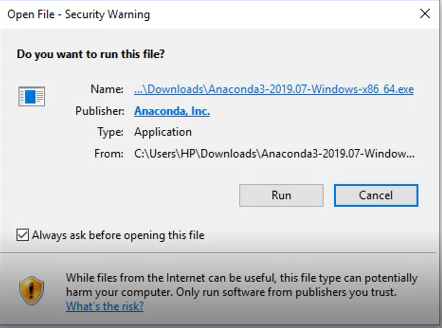
\includegraphics[scale=0.5]{figures/1}}
        \caption{Run Setup Anaconda}
		\label{langkah1}
\end{figure}

\item Tunggu hingga \textit{setup loading} selesai
\begin{figure}[H]
        \centerline{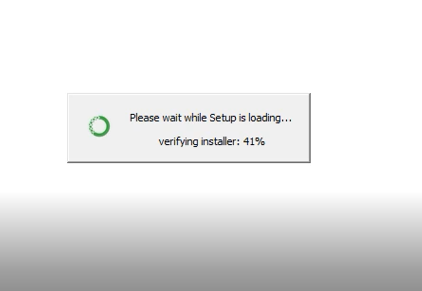
\includegraphics[scale=0.5]{figures/2}}
        \caption{Setup Loading}
		\label{langkah2}
\end{figure}


\item Jika \textit{setup loading} telah selesai, maka klik \textit{next}
\begin{figure}[H]
        \centerline{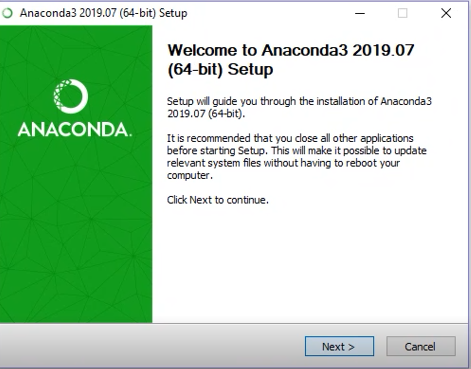
\includegraphics[scale=0.5]{figures/3}}
        \caption{Welcome to Anaconda Setup}
		\label{langkah2}
\end{figure}


\item Pada \textit{License Agreement} klik \textit{I Agree}
 gambar \textit{License Agreement}.

\begin{figure}[H]
    \centering
    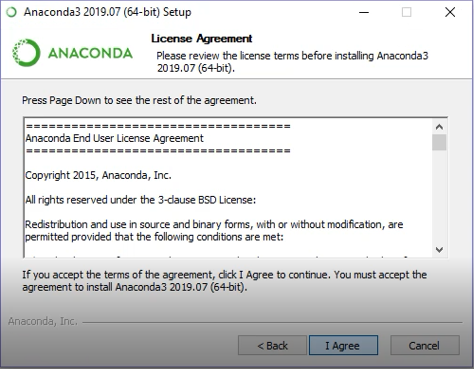
\includegraphics[scale=0.5]{figures/4}
    \caption{\textit{License Agreement}}
    \label{Figureanaconda3}
\end{figure}


\item Kemudian pilih \textit{Just Me(Recomended)} agar sesuai dengan komputer yang digunakan, kemudian klik \textit{next}
 gambar \textit{Just Me(recomended)}.

\begin{figure}[H]
    \centering
    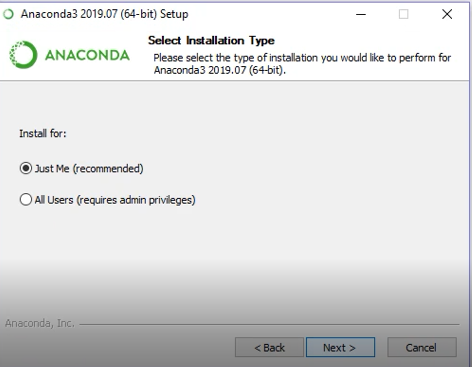
\includegraphics[scale=0.5]{figures/5}
    \caption{\textit{Just Me(recomended)}}
    \label{Figureanaconda4}
\end{figure}


\item Kemudian pilih lokasi tempat \textit{menginstall anaconda}
 gambar \textit{Pilih lokasi}.

\begin{figure}[H]
    \centering
    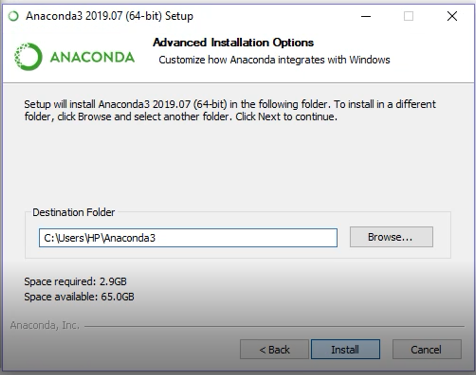
\includegraphics[scale=0.5]{figures/6}
    \caption{\textit{Pilih lokasi}}
    \label{Figureanaconda5}
\end{figure}

\item Kemudian centang \textit{Add Anaconda to my Path environtment variable}, agar saat \textit{menginstall selenium} langsung ke \textit{path anaconda} tidak ke aplikasi yang lain. Klik \textit{install}
 gambar \textit{Centang Anaconda to my PATH}.

\begin{figure}[H]
    \centering
    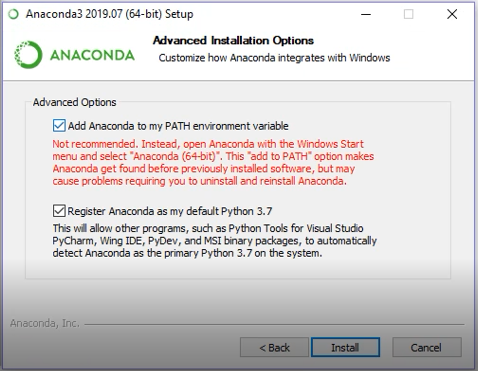
\includegraphics[scale=0.5]{figures/7}
    \caption{\textit{Centang Anaconda to my PATH}}
    \label{Figureanaconda6}
\end{figure}

\item Tunggu sampai proses \textit{installasi} selesai
 gambar \textit{Installation Complete}.

\begin{figure}[H]
    \centering
    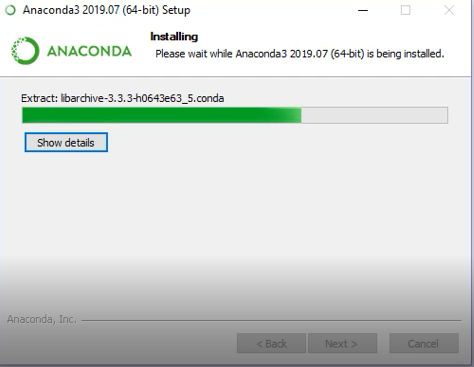
\includegraphics[scale=0.5]{figures/8}
    \caption{\textit{Installation Complete}}
    \label{Figureanaconda7}
\end{figure}

\item Apabila instalasi telah selesai klik \textit{next}
\begin{figure}[H]
    \centering
    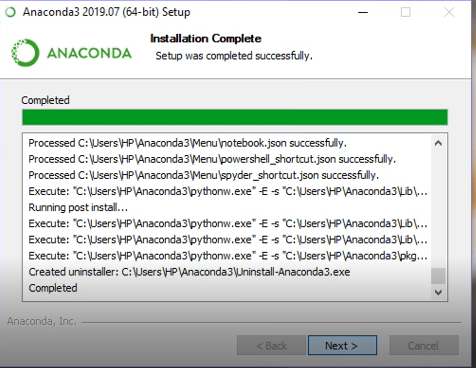
\includegraphics[scale=0.5]{figures/9}
    \caption{\textit{Installation Complete}}
    \label{Figureanaconda8}
\end{figure}

\item klik \textit{next}
\begin{figure}[H]
    \centering
    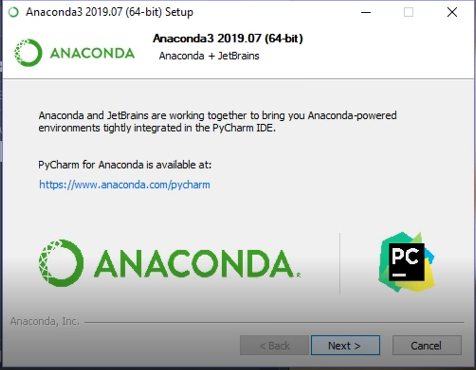
\includegraphics[scale=0.5]{figures/10}
    \caption{\textit{Anaconda+JetBrains}}
    \label{Figureanaconda70}
\end{figure}

\item Jika sudah klik \textit{finish}
 gambar \textit{Thanks fo install Anaconda}.

\begin{figure}[H]
    \centering
    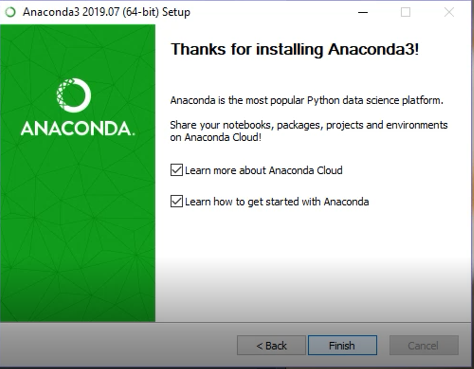
\includegraphics[scale=0.5]{figures/11}
    \caption{\textit{Thanks for install Anaconda}}
    \label{Figureanaconda70}
\end{figure}
\end{enumerate}

\section{Instalasi Pip}

\begin{enumerate}
\item buka anaconda promt
\item ketikkan Pip install selenium
\begin{figure}[H]
    \centering
    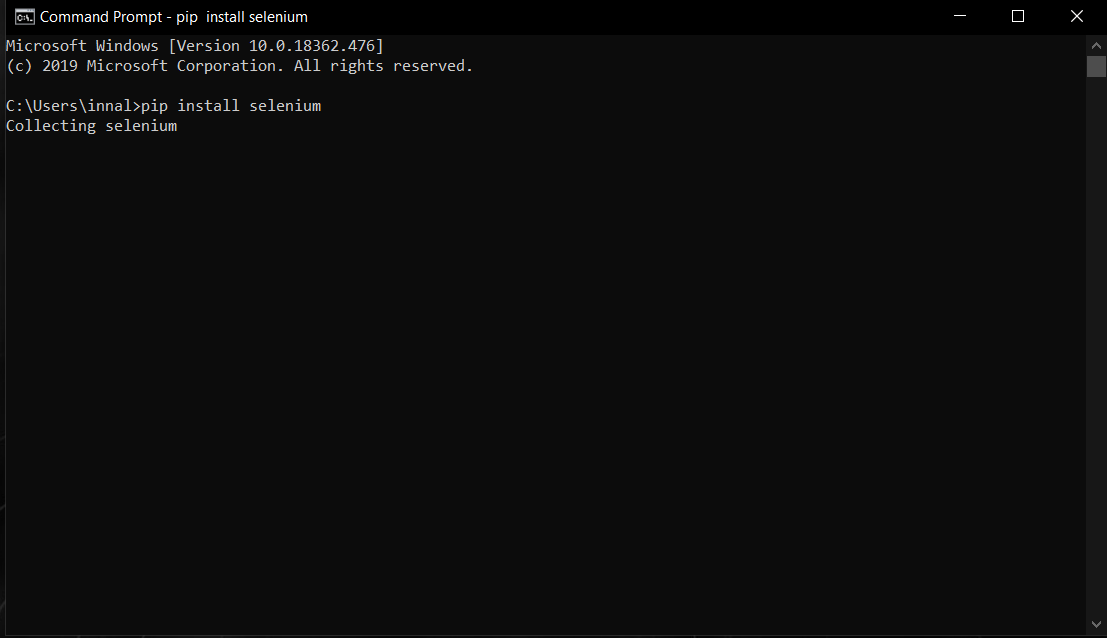
\includegraphics[scale=0.3]{figures/installpip (2)}
    \caption{\textit{Install pip}}
    \label{Figureanaconda70}
\end{figure}
\item Tunggu hingga proses instalasi selesai.
\begin{figure}[H]
    \centering
    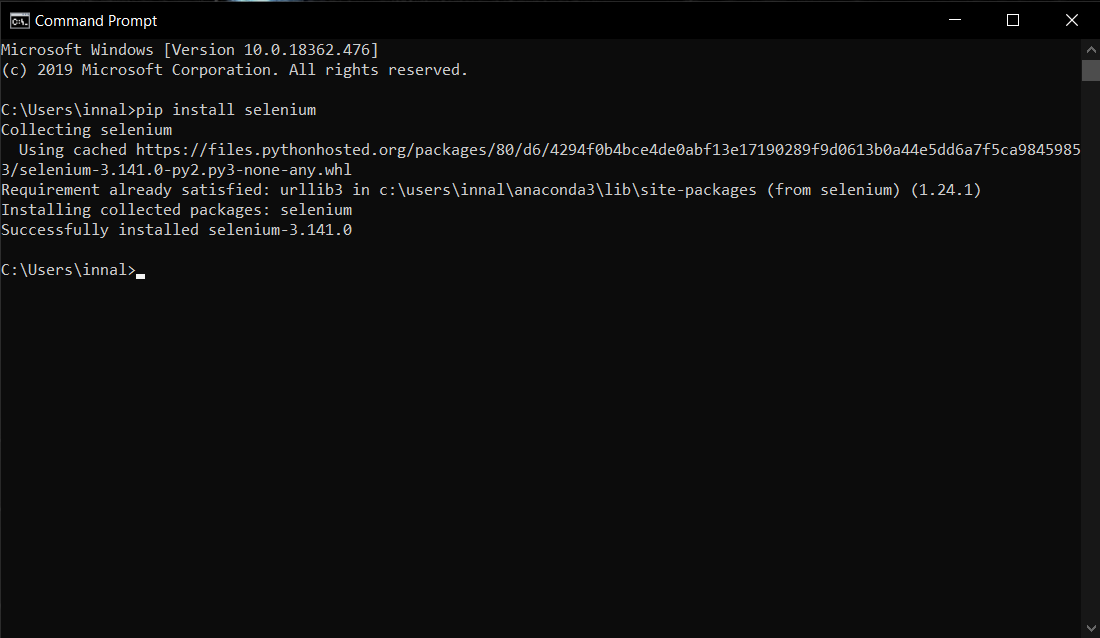
\includegraphics[scale=0.3]{figures/pipselesai (2)}
    \caption{\textit{Install pip Selesai}}
    \label{Figureanaconda70}
\end{figure}
\item jika telah selesai, lakukan pengecekan versi pip dengan mengetikkan pip -V
\begin{figure}[H]
    \centering
    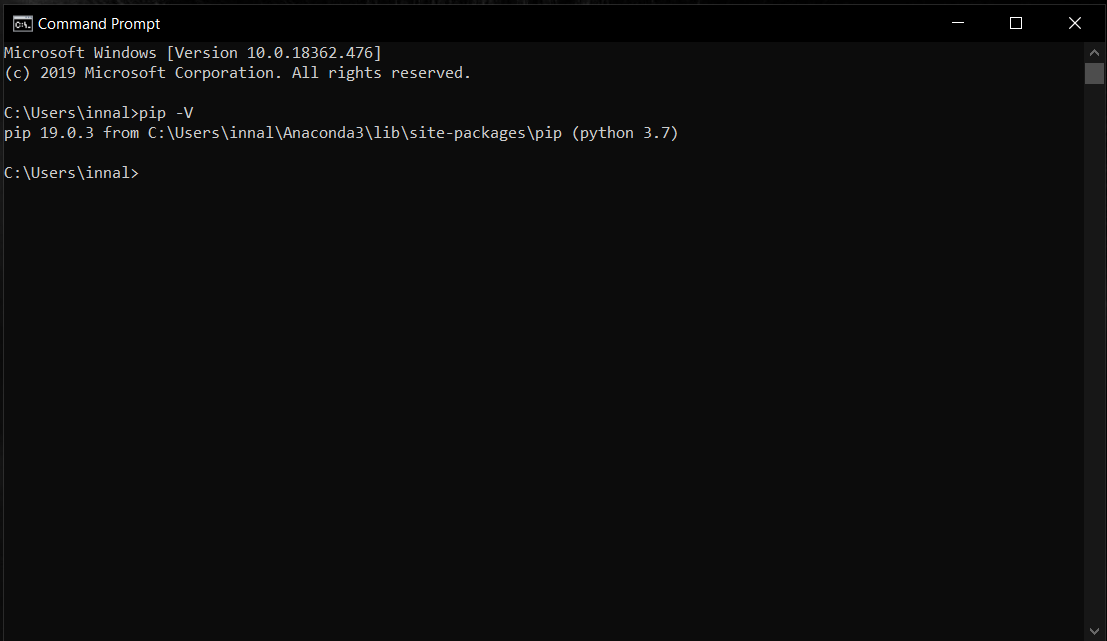
\includegraphics[scale=0.5]{figures/pipversion (2)}
    \caption{\textit{Melihat Versi pip}}
    \label{Figureanaconda70}
\end{figure}

\end{enumerate}

\section{Setting Environment}
\subsection{Windows (Windows 10)}
\begin{enumerate}
\item Buka file explorer
\item Klik kanan pada This pc, lalu pilih properties
\begin{figure}[H]
    \centering
    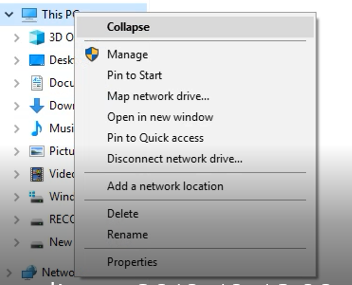
\includegraphics[scale=0.7]{figures/properties}
    \caption{\textit{Properties}}
    \label{Environment1}
\end{figure}
\item Pilih menu Advanced system settings
\begin{figure}[H]
    \centering
    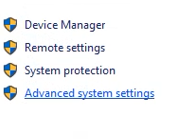
\includegraphics[scale=0.7]{figures/advanced}
    \caption{\textit{Advanced system settings}}
    \label{Environment2}
\end{figure}
\item Pilih Environment Variables
\begin{figure}[H]
    \centering
    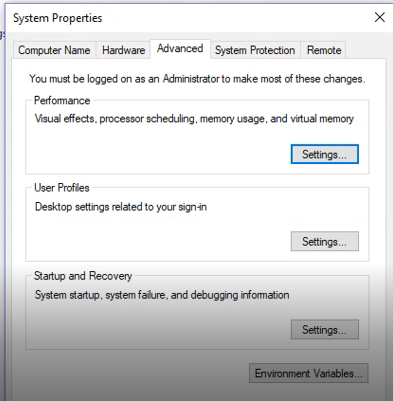
\includegraphics[scale=0.7]{figures/environment}
    \caption{\textit{Environment Variables}}
    \label{Environment3}
\end{figure}
\item Pilih Path, lalu pilih environment variable yang ingin ditambahkan, klik OK
\begin{figure}[H]
    \centering
    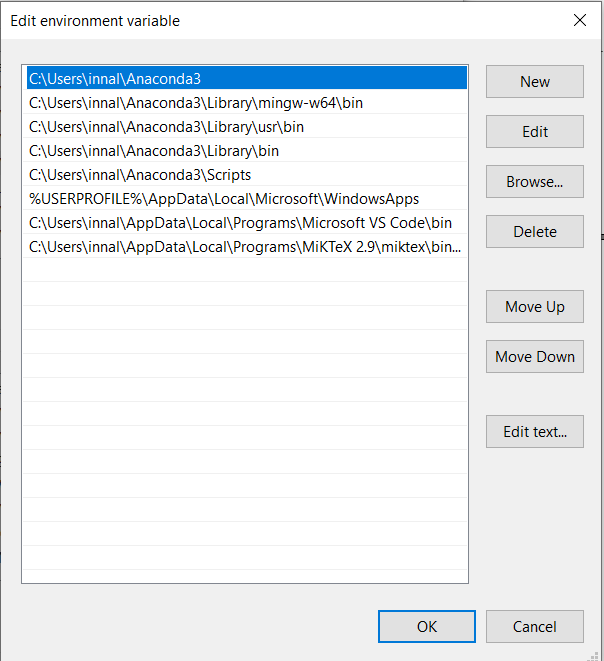
\includegraphics[scale=0.7]{figures/path}
    \caption{\textit{Path}}
    \label{Environment4}
\end{figure}

\end{enumerate}

\section{Geckodriver dan Chromedriver}
\subsection{Gechodriver untuk Mozilla Firefox}
\par Download Geckodriver pada link ini https://github.com/mozilla/geckodriver/releases. sebelum mendownload harus menyamakan versi mozilla dengan versi Geckodriver misal versi Mozilla firefox versi 32bit Geckodrivernya pun harus 32bit jika tidak maka akan terjadi kesalahan.

jika sudah mendownload Geckodriver pindahkan file tersebut ke system32
\begin{figure}[H]
    \centering
    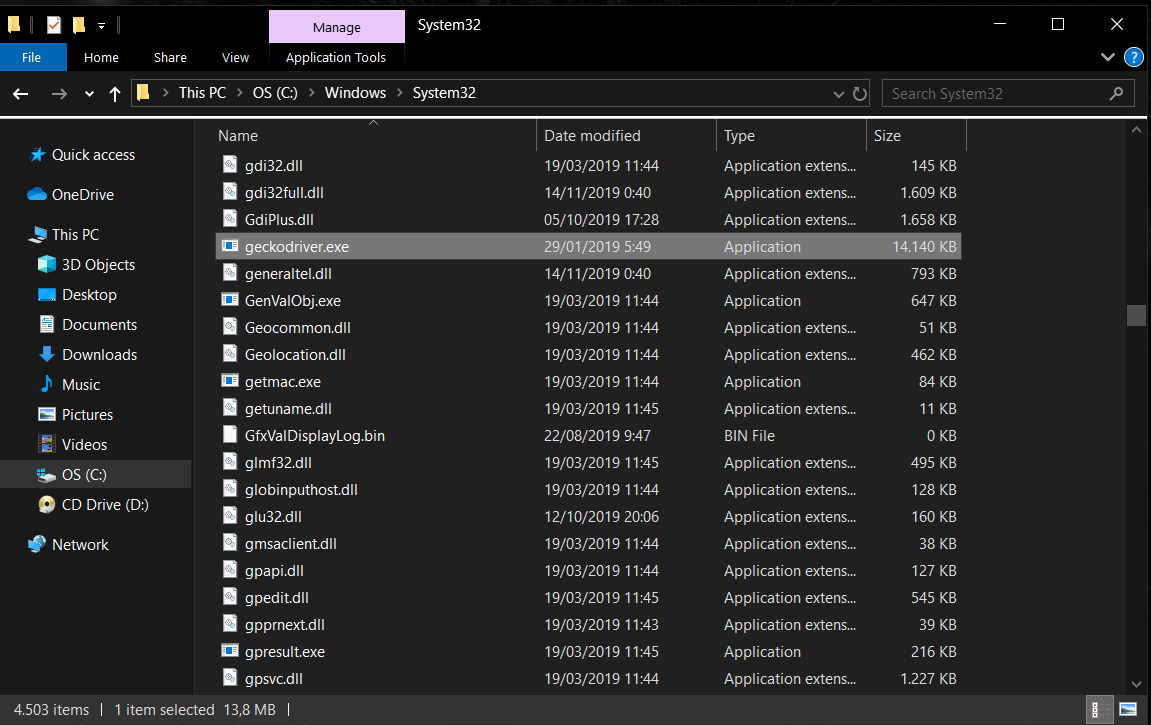
\includegraphics[scale=0.3]{figures/gechodriver}
    \caption{\textit{Gechodriver}}
    \label{Geckodriver}
\end{figure}






\chapter{Menggunakan Selenium}
\section{Penggunaan Selenium}
%\par Disini kami mencoba menjalankan otomasi \textit{web testing} menggunakan \textit{python} dan dengan menggunakan \textit{IDE Spyder}.
%Langkah-langkahnya yaitu :
%\begin{enumerate}
%\item buka \textit{spyder} dan tampilan awalnya seperti ini :
%	\begin{figure}[H]
    	\centering
    	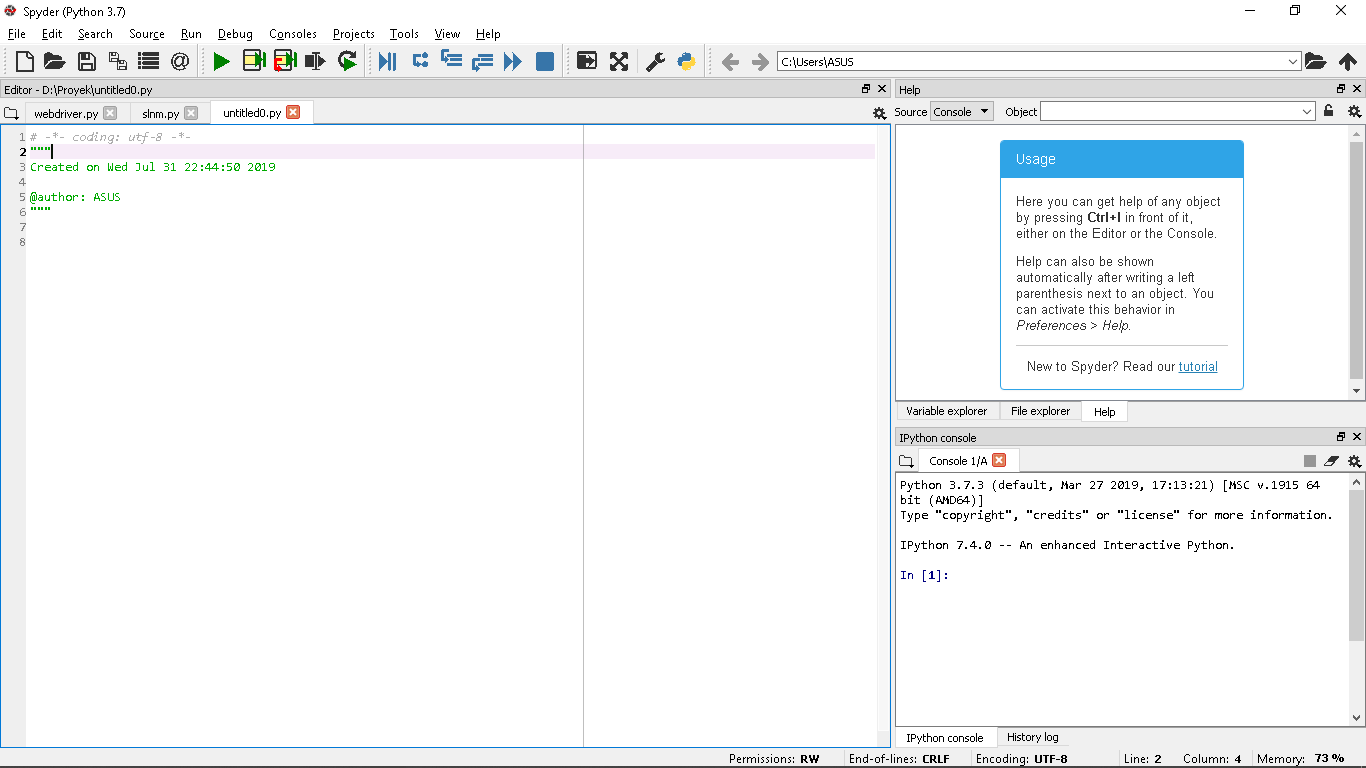
\includegraphics[scale=0.3]{figures/awalspy.png}
    	\caption{\textit{Tampilan awal spyder}}
    	\label{CLI}
	\end{figure}
	
\item kemudian ketikkan codingan :
\begin{lstlisting}[language=Python]
from selenium.webdriver import Firefox
from selenium.webdriver.firefox.options import Options
from selenium.webdriver.common.desired_capabilities import DesiredCapabilities
from selenium.webdriver.firefox.firefox_binary import FirefoxBinary

print("Masukkan Npm Anda:")
npm = input()
print("Masukkan Password SIAP Anda:")
paswd = input('')

opsi = Options()

opsi.headless = False
binary = FirefoxBinary("C:\\Program Files\\Mozilla Firefox\\firefox.exe")
cap = DesiredCapabilities().FIREFOX
cap['marionette'] = True

browser=Firefox(executable_path='geckodriver.exe',
options=opsi,capabilities=cap,firefox_binary=binary)
browser.get('http://siap.poltekpos.ac.id/siap/besan.depan.php')

name = browser.find_element_by_name('user_name')
word = browser.find_element_by_name('user_pass')
login = browser.find_element_by_name('login')


name.send_keys(npm)
word.send_keys(paswd)
login.click()

\end{lstlisting}

Penjelasan Codingan :
\begin{lstlisting}[language=Python]
from selenium.webdriver import Firefox
\end{lstlisting}
Yaitu Modul selenium webdriver mengimplementasikan kelas yang mendukung berbagai browser termasuk Firefox, Chrome, Internet Explorer, Safari, yang lain, dan RemoteWebDri	ver juga untuk menguji pada browser yang tersedia di mesin jarak jauh. Kita perlu mengimpor webdriver dari paket Selenium untuk menggunakan metode Selenium WebDriver.

\begin{lstlisting}[language=Python]
from selenium.webdriver.firefox.options import Options
\end{lstlisting}
Yaitu Opsi kelas dalam paket webdriver selenium firefox. opts adalah turunan dari kelas Opsi yang dipakai untuk program.

\begin{lstlisting}[language=Python]
from selenium.webdriver.common.desired_capabilities import DesiredCapabilities
\end{lstlisting}
Webdriver.common.desired_capabilities import DesiredCapabilities()
sebagai titik awal untuk membuat objek kemampuan yang diinginkan untuk meminta driver web jarak jauh untuk terhubung ke server selenium.

\begin{lstlisting}[language=Python]
from selenium.webdriver.firefox.firefox_binary import FirefoxBinary
\end{lstlisting}
Yaitu untuk mengimport FirefoxBinary atau lokasi dari si firefox.

\begin{lstlisting}[language=Python]
print("Masukkan Npm Anda:")
npm = input()
print("Masukkan Password SIAP Anda:")
paswd = input('')

\end{lstlisting}
ini merupakan inputan \textit{user}

\begin{lstlisting}[language=Python]
browser.get('http://siap.poltekpos.ac.id/siap/besan.depan.php')
\end{lstlisting}
Browser.get metode akan menavigasi ke halaman yang diberikan oleh URL. WebDriver akan menunggu hingga halaman dimuat penuh (yaitu, "onload" telah diaktifkan) sebelum mengembalikan kontrol ke tes atau skrip.

\item Setelah membuat Tambahan Codingan  seperti diatas untuk merunning program anda tekan run pada bar diatas.
\begin{figure}[H]
    	\centering
    	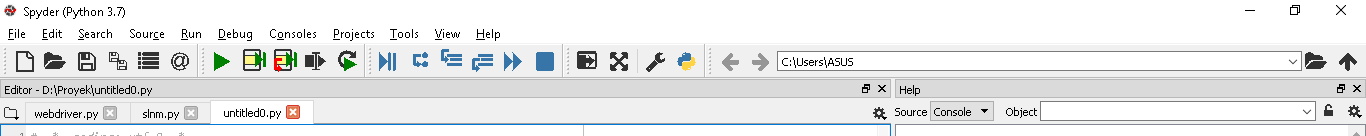
\includegraphics[scale=0.3]{figures/run1.png}
    	\caption{\textit{Running spyder}}
    	\label{CLI}
	\end{figure}

\newpage

\item Pada saat di run akan terlihat pada IPython console seperti gambar 
\begin{figure}[H]
    	\centering
    	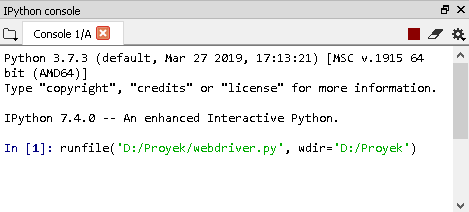
\includegraphics[scale=0.5]{figures/run2.png}
    	\caption{\textit{Running spyder console}}
    	\label{CLI}
	\end{figure}

\item Saat kotak yang ditandai pada gambar dibawah, berwarna merah artinya proses running program tersebut masih berjalan.
\begin{figure}[H]
    	\centering
    	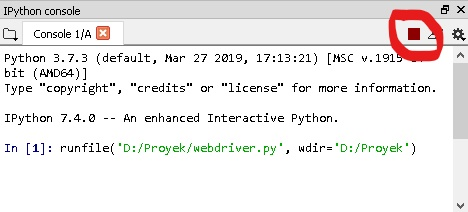
\includegraphics[scale=0.5]{figures/run3.png}
    	\caption{\textit{Running masih berjalan}}
    	\label{CLI}
	\end{figure}

\item Jika proses \textit{running} sudah selesai tampilannya akan seperti ini. Berarti Tambahan Codingan tersebut berhasil di \textit{running} dan tidak terdapat \textit{error}.
\begin{figure}[H]
    	\centering
    	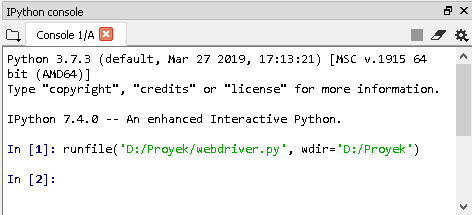
\includegraphics[scale=0.5]{figures/run4.png}
    	\caption{\textit{Running selesai}}
    	\label{CLI}
	\end{figure}

\item Setelah program di run akan otomatis membuka Mozila Firefox dan akan langsung membuka website siap.poltekpos.ac.id secara otomatis.
\begin{figure}[H]
    	\centering
    	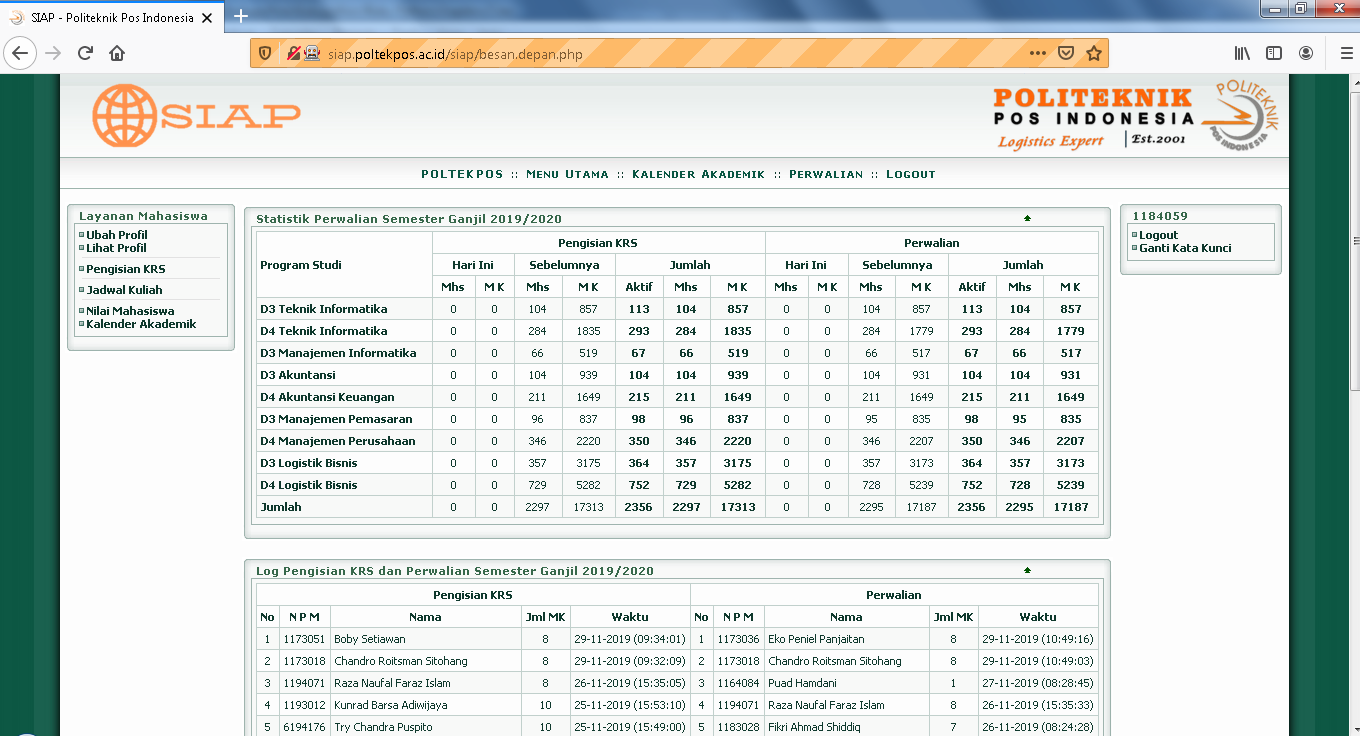
\includegraphics[scale=0.3]{figures/run5.png}
    	\caption{\textit{Tampilan siap.poltekpos}}
    	\label{CLI}
	\end{figure}


\end{enumerate}

\subsection{Cara find element atau class }
\par Selanjutnya kami akan mencoba \textit{Find Element} yang terdapat pada \textit{website} tersebut. Sebelumnya anda harus mengetahui apa saja jenis-jenis \textit{element} dan berikut adalah contoh dari \textit{element}.

\begin{enumerate}
\item find_element_by_id
\par Gunakan ini ketika Anda tahu atribut id suatu elemen. Dengan strategi ini, elemen pertama dengan nilai atribut id yang cocok dengan lokasi akan dikembalikan.
contoh :
\begin{lstlisting}[language=Python]
<form id="login">
   login = Browser.find_element_by_id('login')
\end{lstlisting}

\item find_element_by_name
\par Gunakan ini ketika Anda tahu atribut nama elemen. Dengan strategi ini, elemen pertama dengan nilai atribut nama yang cocok dengan lokasi akan dikembalikan.
contoh :
\begin{lstlisting}[language=Python]
<input name ="username" type="text" />
  username = Browser.find_element_by_name('username')
\end{lstlisting}

\item find_element_by_xpath
\par XPath adalah bahasa yang digunakan untuk menemukan node dalam dokumen XML. Karena HTML dapat menjadi implementasi XML (XHTML), pengguna Selenium dapat memanfaatkan bahasa yang kuat ini untuk menargetkan elemen dalam aplikasi web mereka. Dan cara mendapatkan xpath adalah inspect website tersebut dan klik kanan pada element yang ingin di cari dan klik copy dan disana ada copy Xpath.
contoh :
\begin{lstlisting}[language=Python]
" ('/html/body/table/tbody/tr[5]/td/table[3]/tbody/tr[1]/td[2]/p[1]/table/tbody/tr/td[3]/select').click()" 
 browser.find_element_by_xpath('/html/body/table/tbody/tr[5]/td/table[3]/tbody/tr[1]/td[2]/p[1]/table/tbody/tr/td[3]/select').click()
\end{lstlisting}

\item find_element_by_link_text
\par Gunakan ini ketika Anda tahu teks tautan yang digunakan dalam tag jangkar. Dengan strategi ini, elemen pertama dengan nilai teks tautan yang cocok dengan lokasi akan dikembalikan. 
contoh :
\begin{lstlisting}[language=Python]
<a href="continue.html">Continue</a>
Continue = Browser.find_element_by_link_text('Continue')
\end{lstlisting}

\item find_element_by_tag_name
\par Gunakan ini ketika Anda ingin mencari elemen dengan nama tag. Dengan strategi ini, elemen pertama dengan nama tag yang diberikan akan dikembalikan.
contoh :
\begin{lstlisting}[language=Python]
<strong>Hello</strong> 
Strong = Browser.find_element_by_tag_name('strong')
\end{lstlisting}

\item find_element_by_class_name
\par Gunakan ini ketika Anda ingin mencari elemen dengan nama atribut kelas. Dengan strategi ini, elemen pertama dengan nama atribut kelas yang cocok akan dikembalikan. 
contoh :
\begin{lstlisting}[language=Python]
<p class="body">Halo.</p>
body = Browser.find_element_by_class_name('body')
\end{lstlisting}

\item find_element_by_css_selector
\par Gunakan ini ketika Anda ingin mencari elemen dengan sintaks pemilih CSS. Dengan strategi ini, elemen pertama dengan pemilih CSS yang cocok akan dikembalikan. 
contoh : 
\begin{lstlisting}[language=Python]
<p class="body">Halo.</p> 
body = Browser.find_element_by_class_name('p.body')
\end{lstlisting}

\end{enumerate}

\subsection{Mengambil element dari web siap.poltekpos.ac.id}
\par Setelah mengenal tentang element mari kita mencoba mencari element pada website siap.poltekpos.ac.id

\newpage

\begin{enumerate}
\item Disini kami mencoba untuk mengisi data \textit{user} pada \textit{login}.
\begin{figure}[H]
    	\centering
    	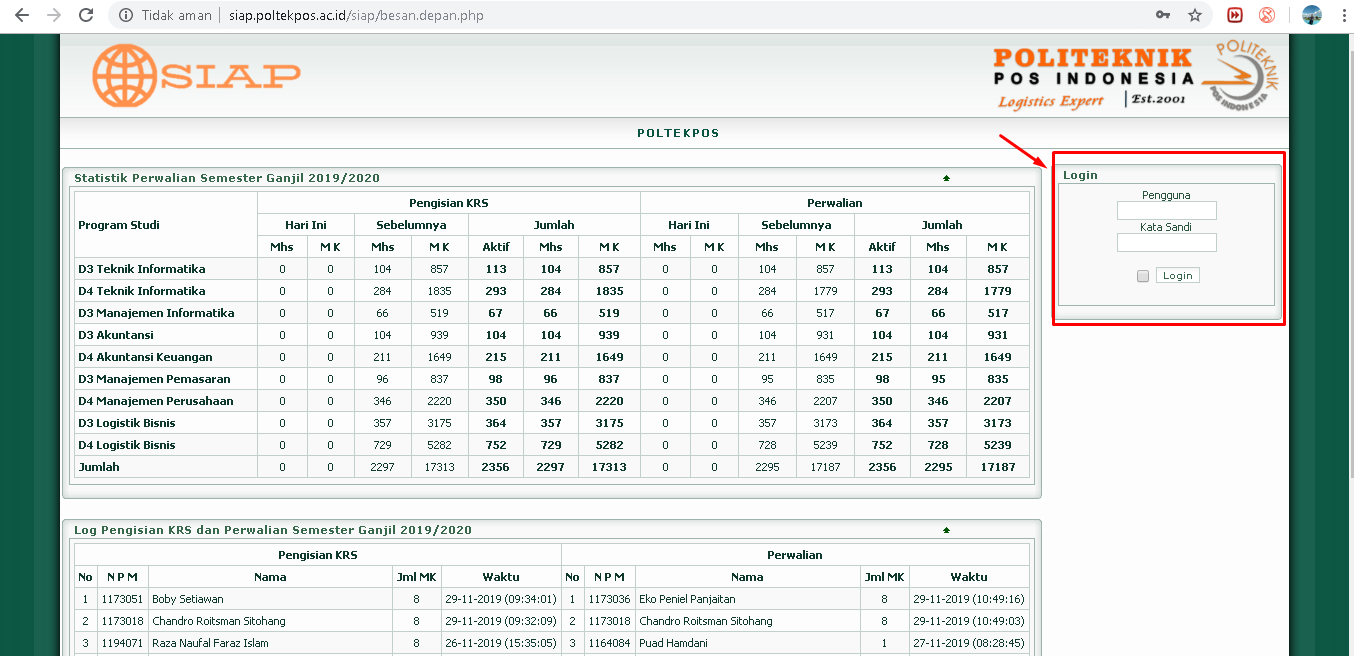
\includegraphics[scale=0.3]{figures/siap.png}
    	\caption{\textit{Tampilan siap.poltekpos}}
    	\label{CLI}
	\end{figure}
\item Untuk mencari elementnya arahkan cursor ke \textit{login} pengguna, kata sandi, dan login. lalu klik kanan dan \textit{inspect}, disini kami menggunakan element_by_name.

\begin{figure}[H]
    	\centering
    	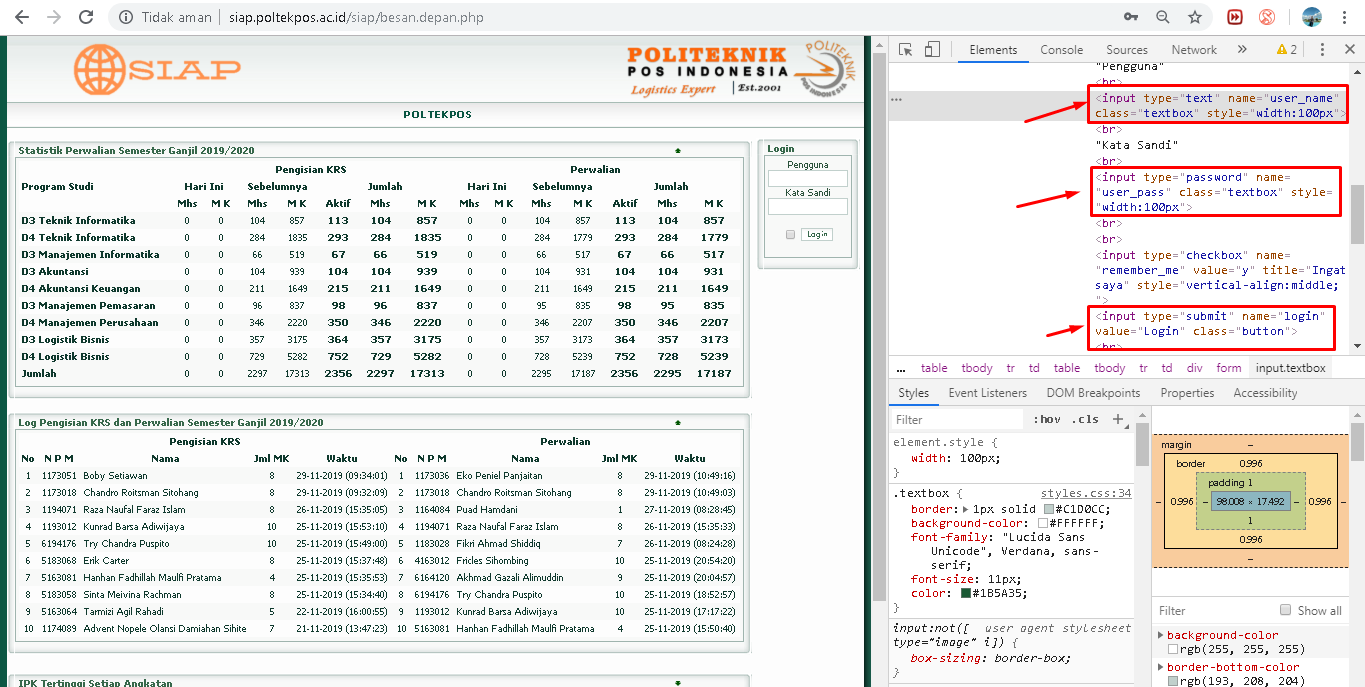
\includegraphics[scale=0.3]{figures/inspect1.png}
    	\caption{\textit{inspect element by name}}
    	\label{CLI}
	\end{figure}
	
Tambahan Codingan :
\begin{lstlisting}[language=Python]
name = browser.find_element_by_name('user_name')
word = browser.find_element_by_name('user_pass')
login = browser.find_element_by_name('login')

\end{lstlisting}

\newpage

Hasil :
\begin{figure}[H]
    	\centering
    	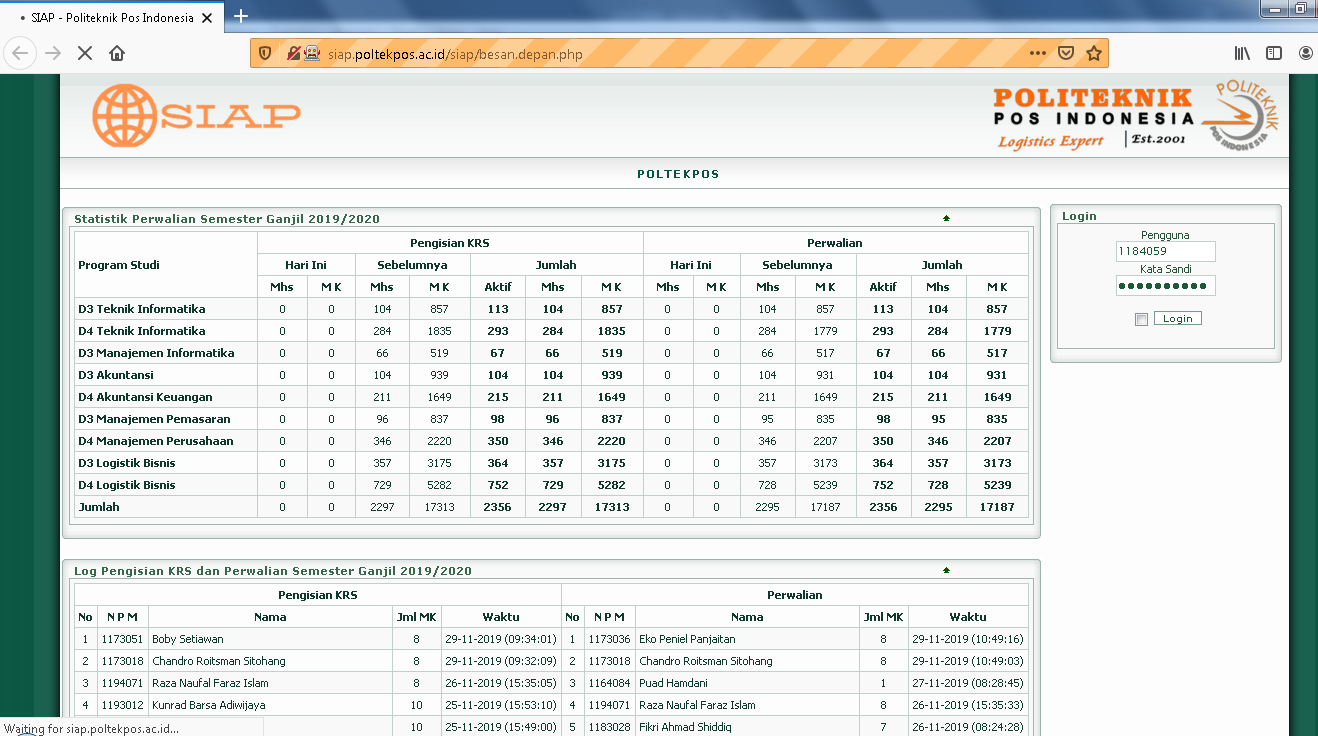
\includegraphics[scale=0.3]{figures/hasillogin.png}
    	\caption{\textit{Tampilan loading login}}
    	\label{CLI}
	\end{figure}
	
Hasil :
\begin{figure}[H]
    	\centering
    	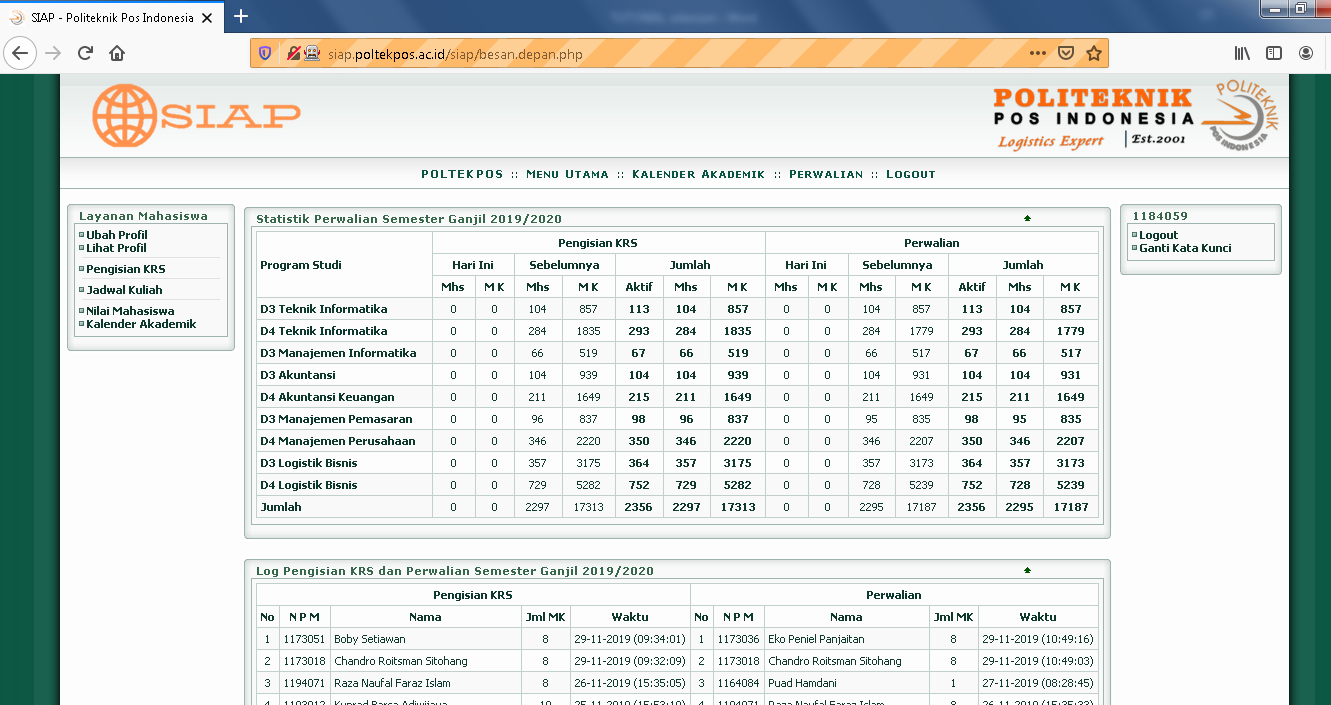
\includegraphics[scale=0.3]{figures/hasillogin1.png}
    	\caption{\textit{Tampilan login}}
    	\label{CLI}
	\end{figure}


\item Pada layanan mahasiswa, kami mencoba untuk melihat nilai mahasiswa secara otomatis. Dengan cara yaitu klik kanan pada nilai mahasiswa, kemudian pilih \textit{inspect}.
\begin{figure}[H]
    	\centering
    	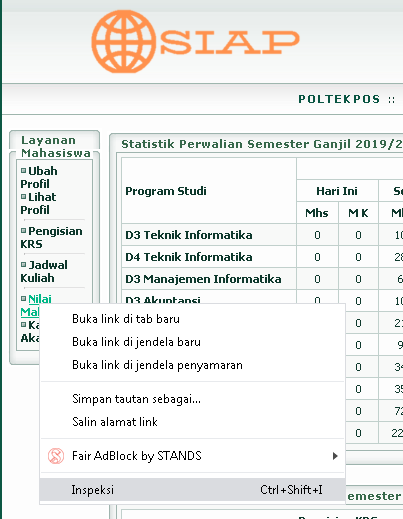
\includegraphics[scale=0.5]{figures/nilai1.png}
    	\caption{\textit{inspect element nilai mahasiswa}}
    	\label{CLI}
	\end{figure}

\newpage

Disini kami mengambil \textit{element by xpath}
\begin{figure}[H]
    	\centering
    	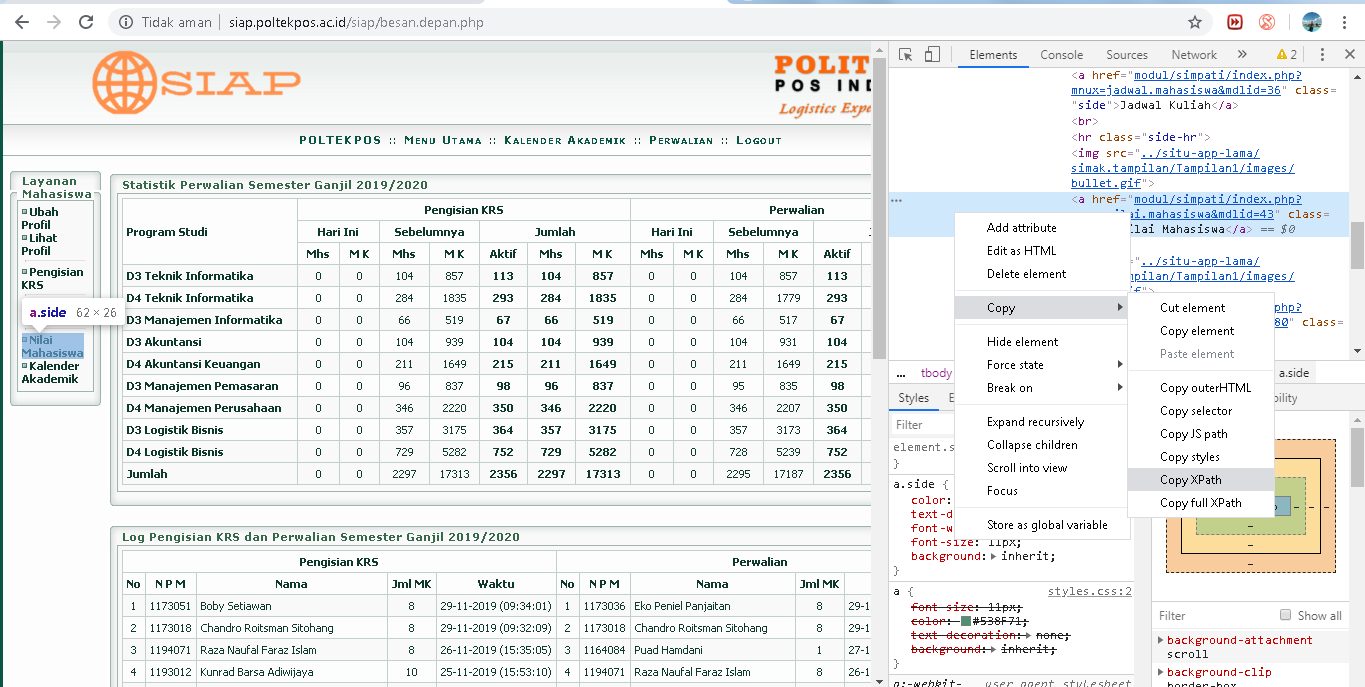
\includegraphics[scale=0.3]{figures/nilai2.png}
    	\caption{\textit{inspect element by xpath}}
    	\label{CLI}
	\end{figure}
	
Tambahan codingan :
\begin{lstlisting}[language=Python]
nilai= browser.find_element_by_xpath("/html/body/table/tbody/tr[5]/td/table[1]/tbody/tr/td[1]/table[2]/tbody/tr[1]/td[2]/a[5]").click()
\end{lstlisting}

Hasil :
\begin{figure}[H]
    	\centering
    	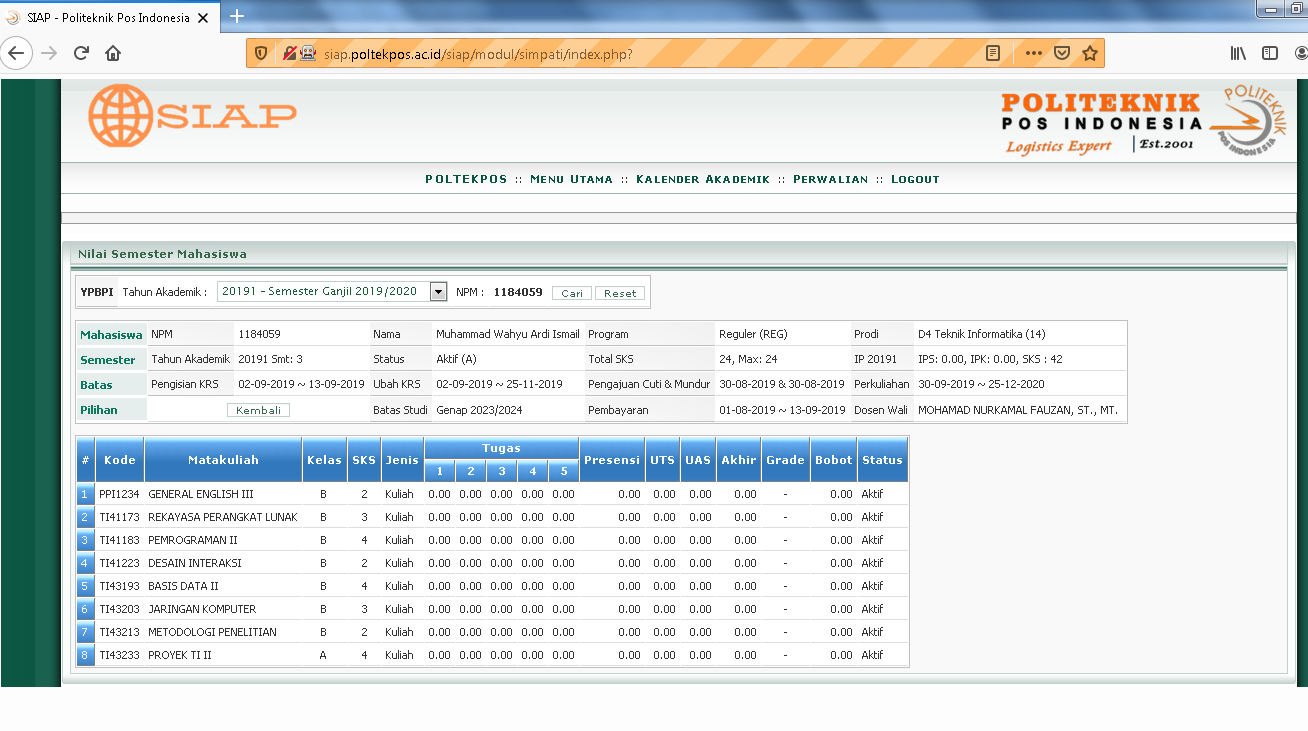
\includegraphics[scale=0.3]{figures/hasilnilai1.png}
    	\caption{\textit{Tampilan nilai semester mahasiswa}}
    	\label{CLI}
	\end{figure}

\newpage
	
\item Kemudian pada kolom tahun akademik, klik kanan dan pilih \textit{inspect}
\begin{figure}[H]
    	\centering
    	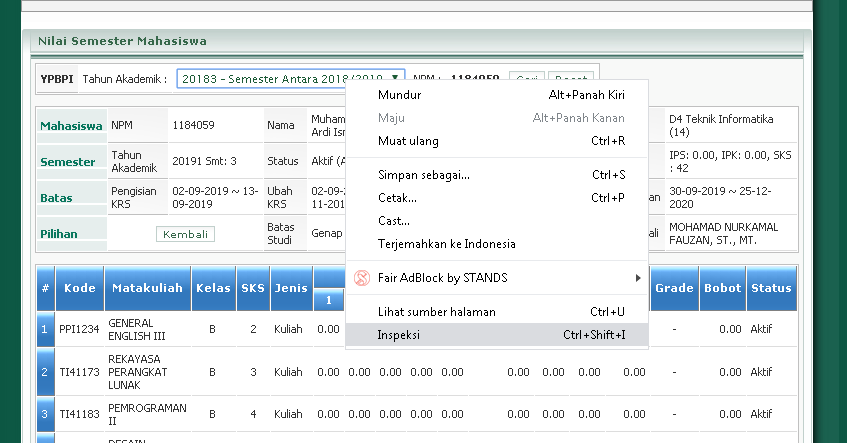
\includegraphics[scale=0.3]{figures/tahun1.png}
    	\caption{\textit{inspect element tahun akademik}}
    	\label{CLI}
	\end{figure}
	
Disini kami mengambil \textit{element by xpath} pada semester genap 2018/2019
\begin{figure}[H]
    	\centering
    	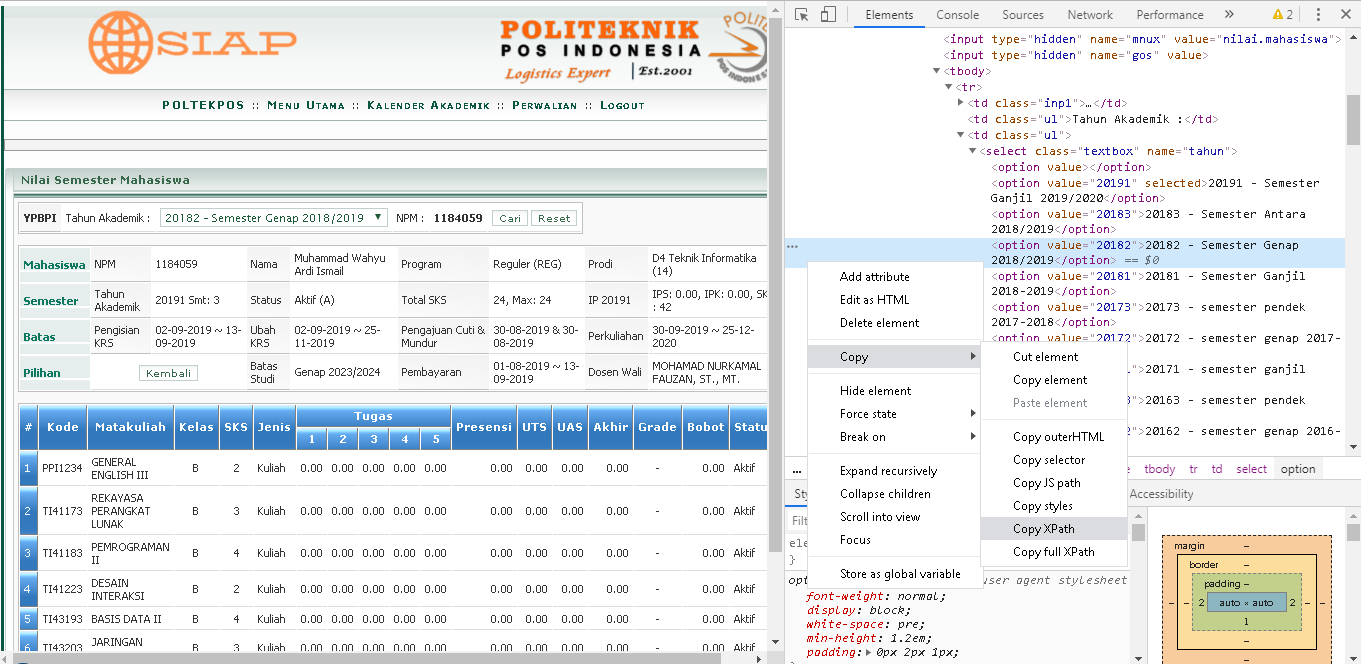
\includegraphics[scale=0.3]{figures/semestergenap.png}
    	\caption{\textit{inspect element by xpath semster genap}}
    	\label{CLI}
	\end{figure}

Tambahan codingan :
\begin{lstlisting}[language=Python]
nilai semester genap =browser.find_element_by_xpath('/html/body/table/tbody/tr[5]/td/table[3]/tbody/tr[1]/td[2]/p[1]/table/tbody/tr/td[3]/select/option[4]').click()
\end{lstlisting}

\newpage

Hasil :
\begin{figure}[H]
    	\centering
    	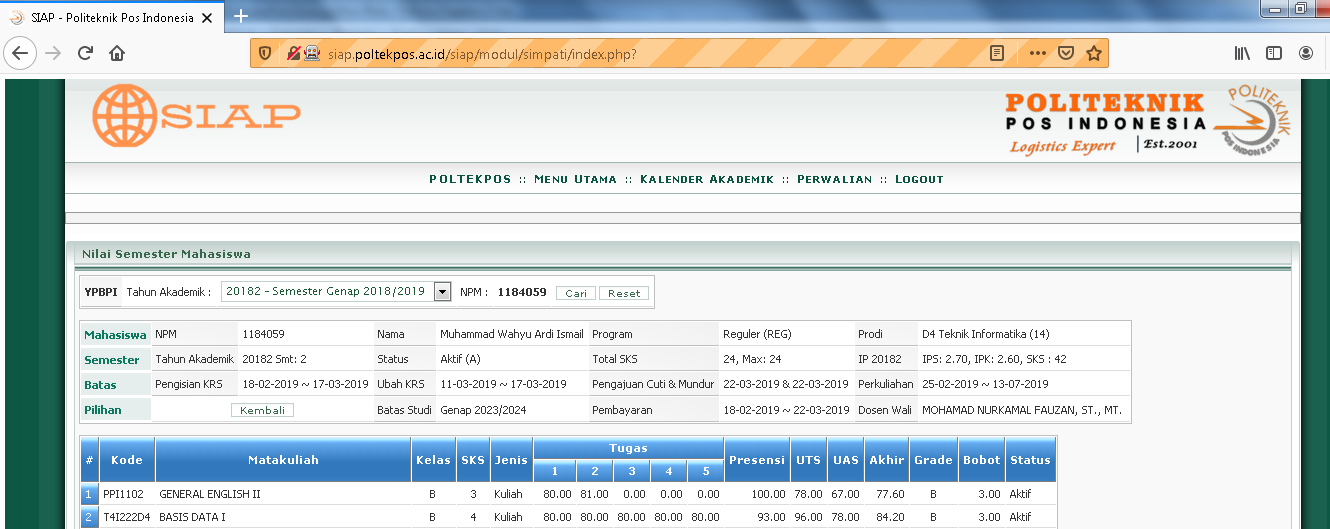
\includegraphics[scale=0.3]{figures/hasilnilai2.png}
    	\caption{\textit{Tampilan nilai semester genap 2018/2019}}
    	\label{CLI}
	\end{figure}



\item kemudian klik find cari dengan cara klik kanan pilih \textit{inspect}
\begin{figure}[H]
    	\centering
    	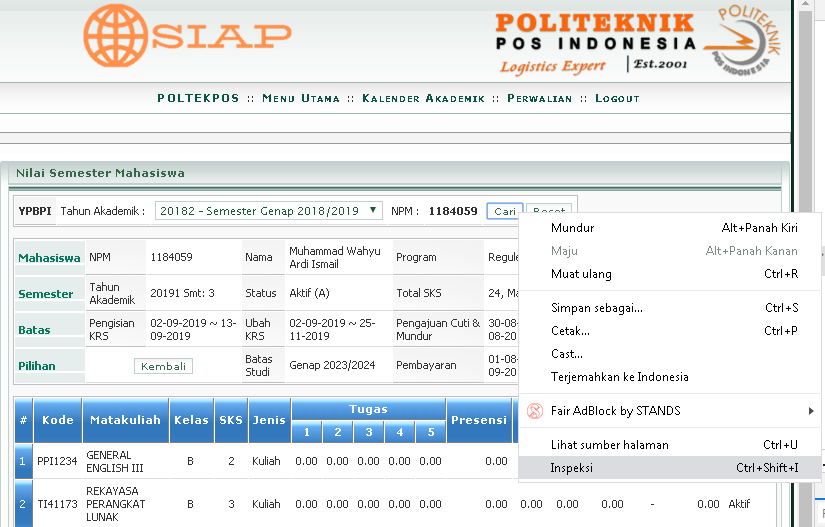
\includegraphics[scale=0.3]{figures/cari1.png}
    	\caption{\textit{inspect element cari}}
    	\label{CLI}
	\end{figure}
	
Disini kami mengambil \textit{element by class name}, \textit{class name} yaitu \textit{button}.
\begin{figure}[H]
    	\centering
    	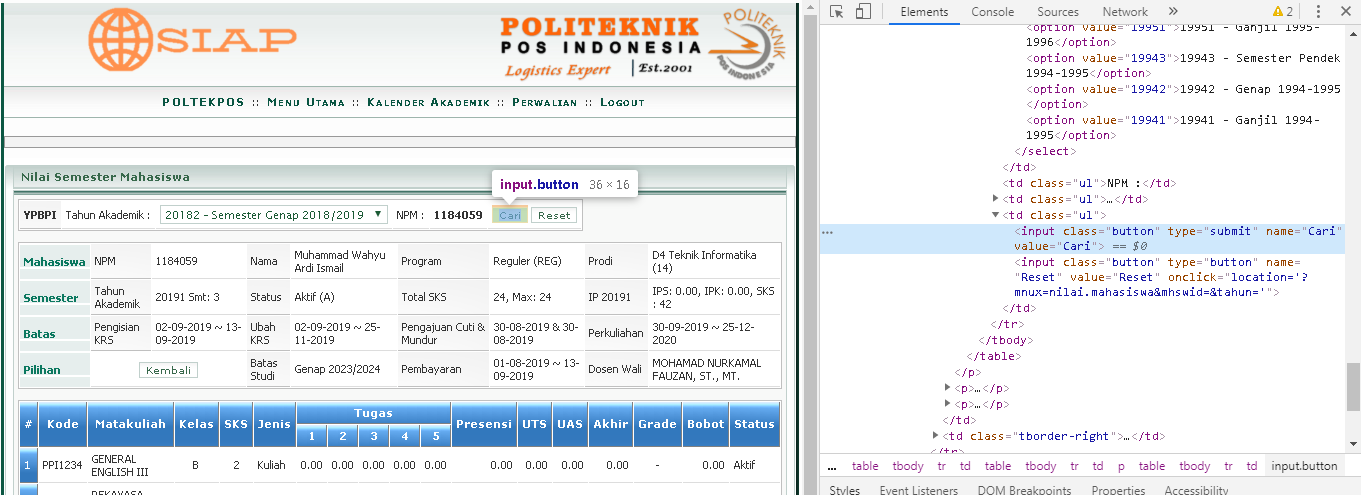
\includegraphics[scale=0.3]{figures/button1.png}
    	\caption{\textit{inspect element by class name cari}}
    	\label{CLI}
	\end{figure}

Tambahan codingan :
\begin{lstlisting}[language=Python]
cari = browser.find_element_by_class_name('button').click()
\end{lstlisting}


\item codingan keseluruhan :
\begin{lstlisting}[language=Python]
from selenium.webdriver import Firefox
from selenium.webdriver.firefox.options import Options
from selenium.webdriver.common.desired_capabilities import DesiredCapabilities
from selenium.webdriver.firefox.firefox_binary import FirefoxBinary

print("Masukkan Npm Anda:")
npm = input()
print("Masukkan Password SIAP Anda:")
paswd = input('')

opsi = Options()

opsi.headless = False
binary = FirefoxBinary("C:\\Program Files\\Mozilla Firefox\\firefox.exe")
cap = DesiredCapabilities().FIREFOX
cap['marionette'] = True

browser=Firefox(executable_path='geckodriver.exe',
options=opsi,capabilities=cap,firefox_binary=binary)
browser.get('http://siap.poltekpos.ac.id/siap/besan.depan.php')

name = browser.find_element_by_name('user_name')
word = browser.find_element_by_name('user_pass')
login = browser.find_element_by_name('login')


name.send_keys(npm)
word.send_keys(paswd)
login.click()

nilai = browser.find_element_by_xpath("/html/body/table/tbody/tr[5]/td/table[1]/tbody/tr/td[1]/table[2]/tbody/tr[1]/td[2]/a[5]").click()
semester1 = browser.find_element_by_xpath('/html/body/table/tbody/tr[5]/td/table[3]/tbody/tr[1]/td[2]/p[1]/table/tbody/tr/td[3]/select/option[4]').click()
cari = browser.find_element_by_class_name('button').click()

\end{lstlisting}


\end{enumerate}


 














%\chapter{Penanganan Error}
%\section{Cara penggunaan}

\begin{figure}[H]
\centering
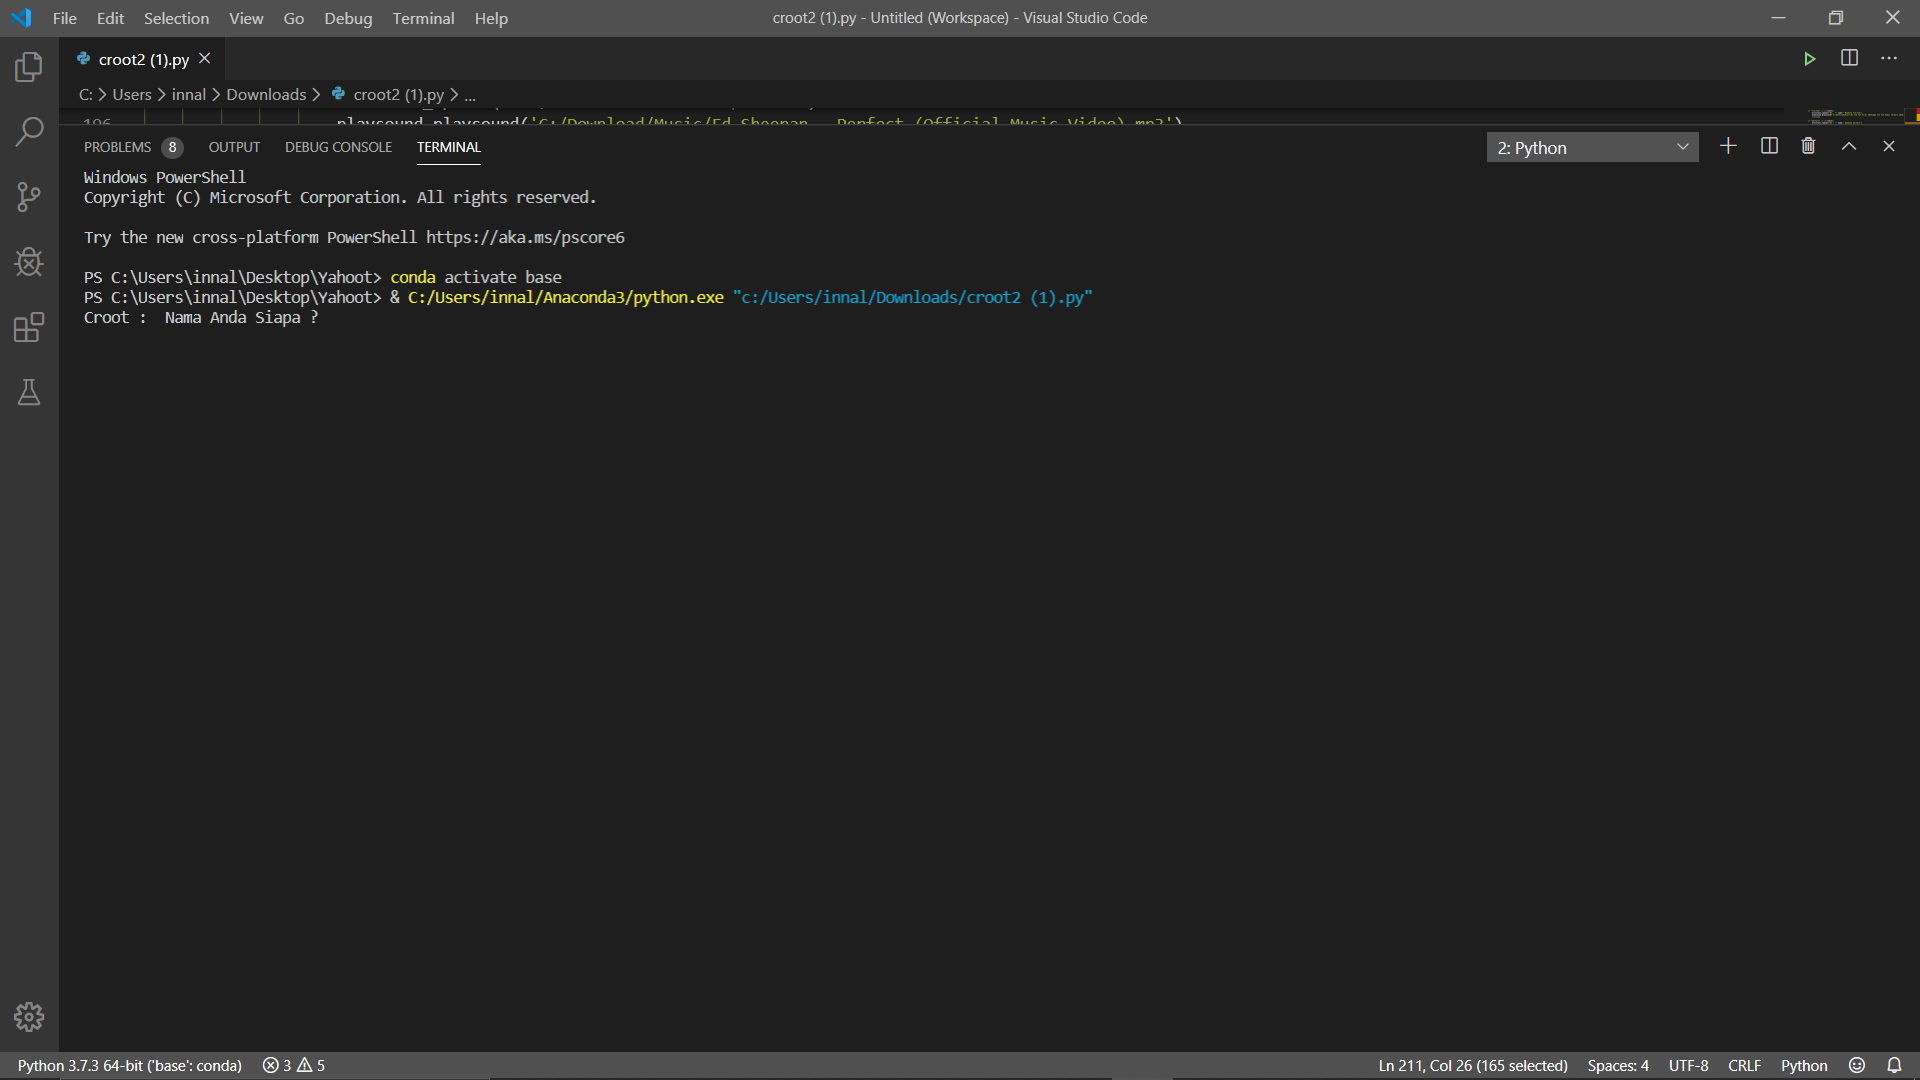
\includegraphics[width=1\textwidth]{tutorial selenium/figures/4q.png}
\caption{}
\label{unicodeuni}
\end{figure}
s
\\
\\
\\
\\
\\
s
\begin{figure}[H]
\centering
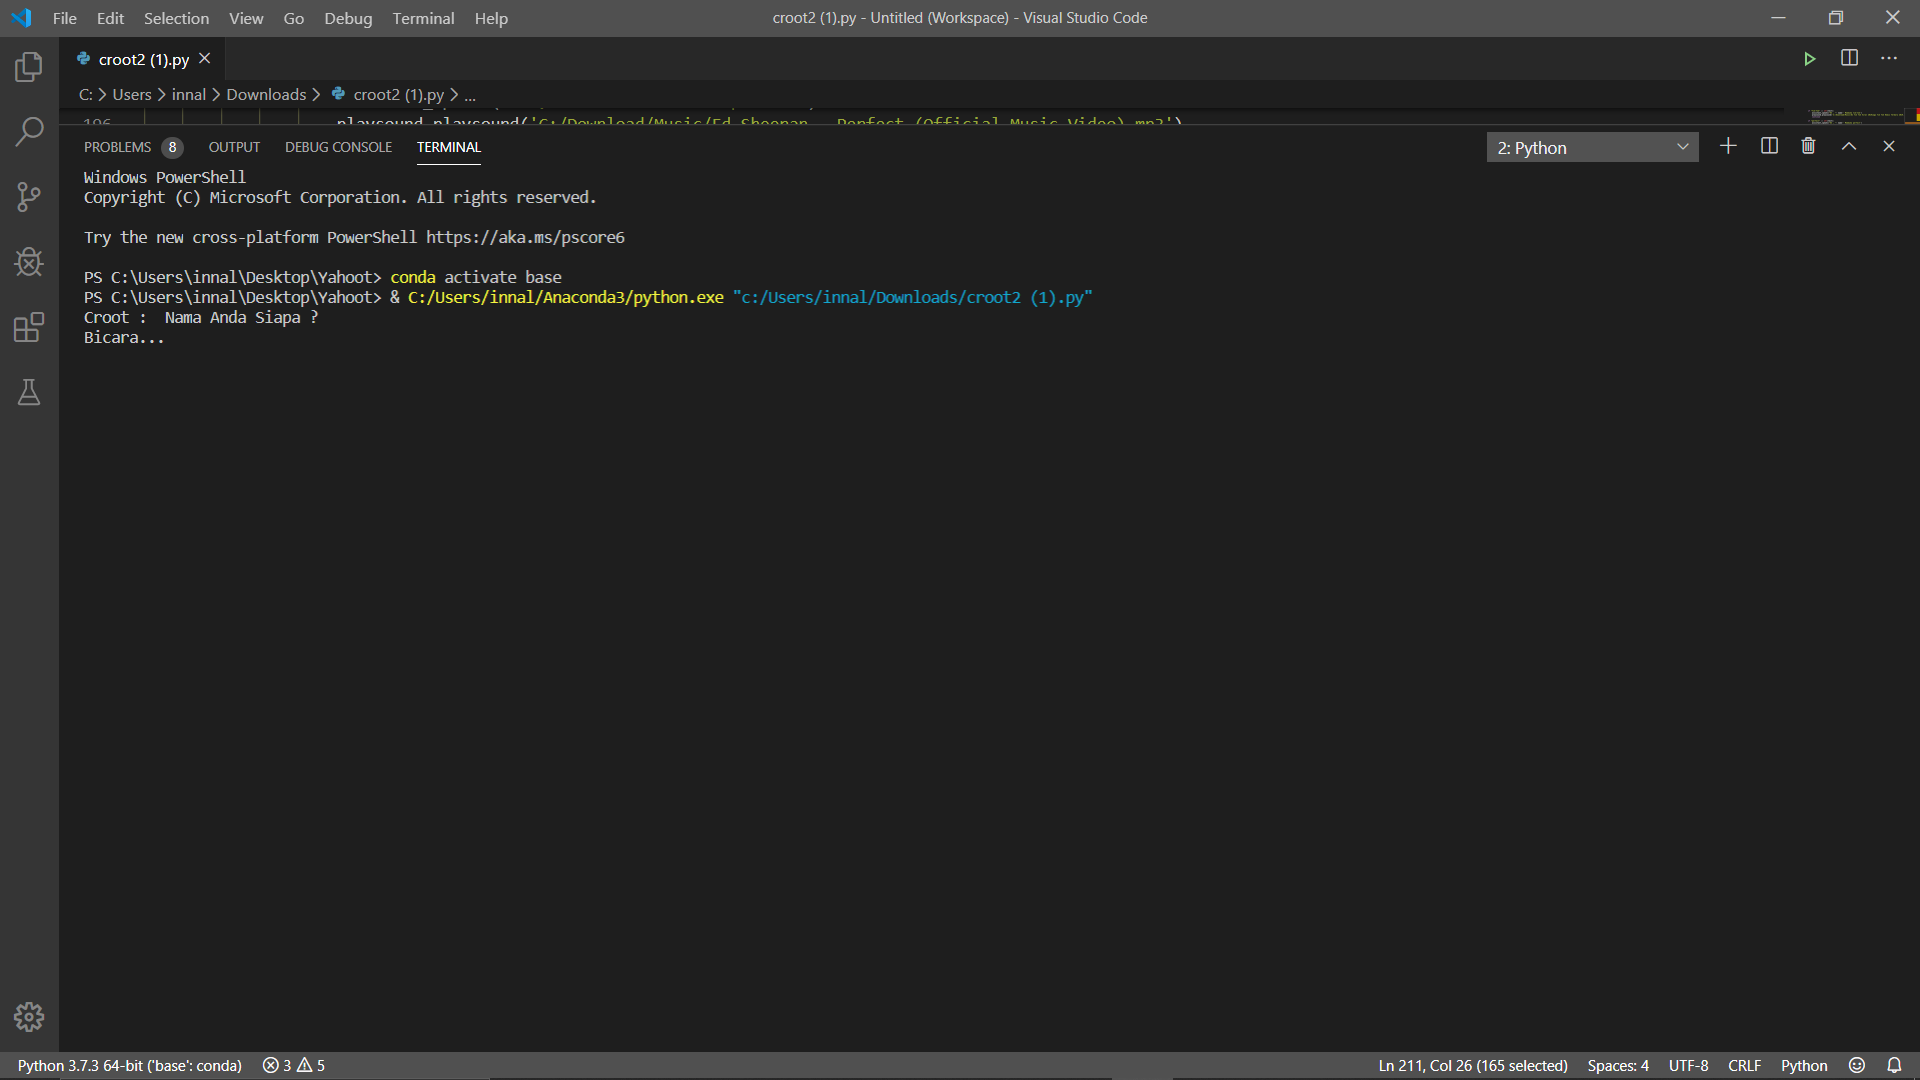
\includegraphics[width=1\textwidth]{tutorial selenium/figures/5q.png}
\caption{}
\label{}
\end{figure}
s
\\
\\
\\
\\
\\
s
\begin{figure}[H]
\centering
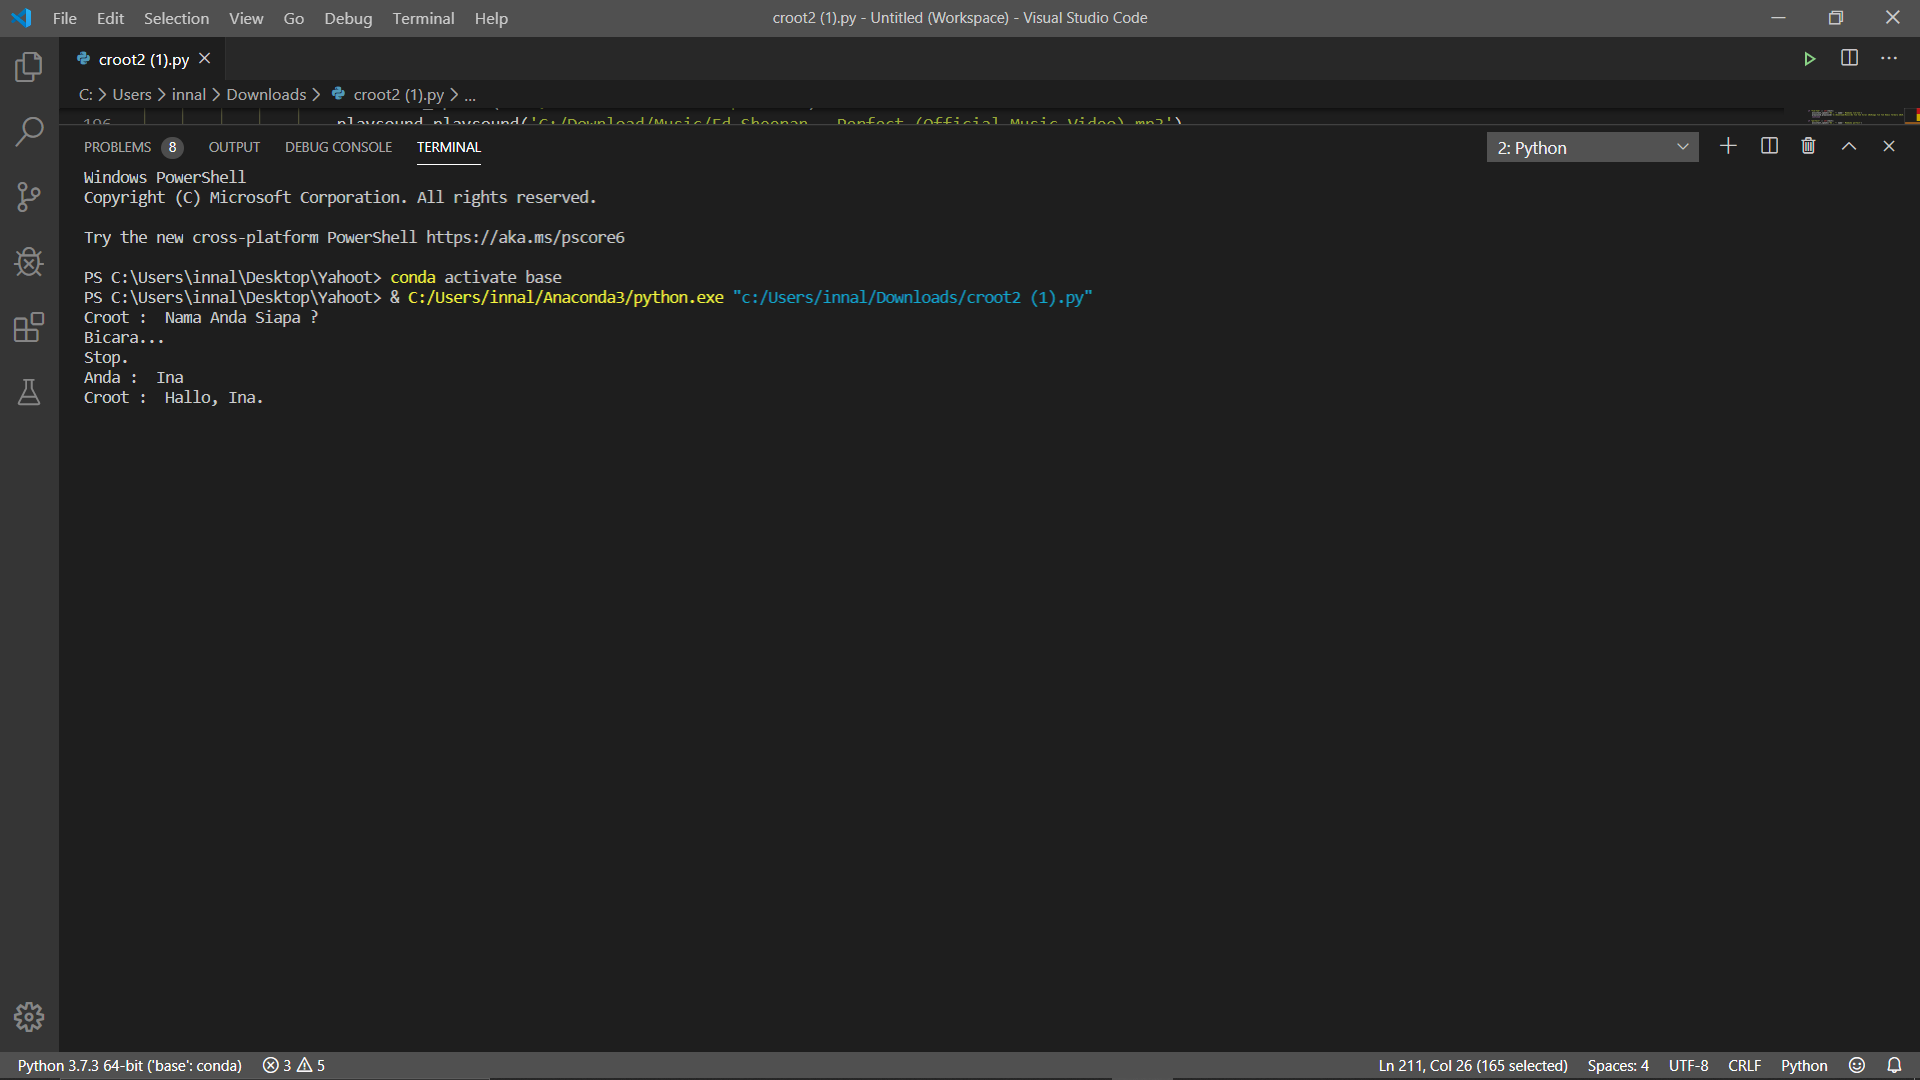
\includegraphics[width=1\textwidth]{tutorial selenium/figures/6q.png}
\caption{}
\label{}
\end{figure}
s
\\
\\
\\
\\
\\
s
\begin{figure}[H]
\centering
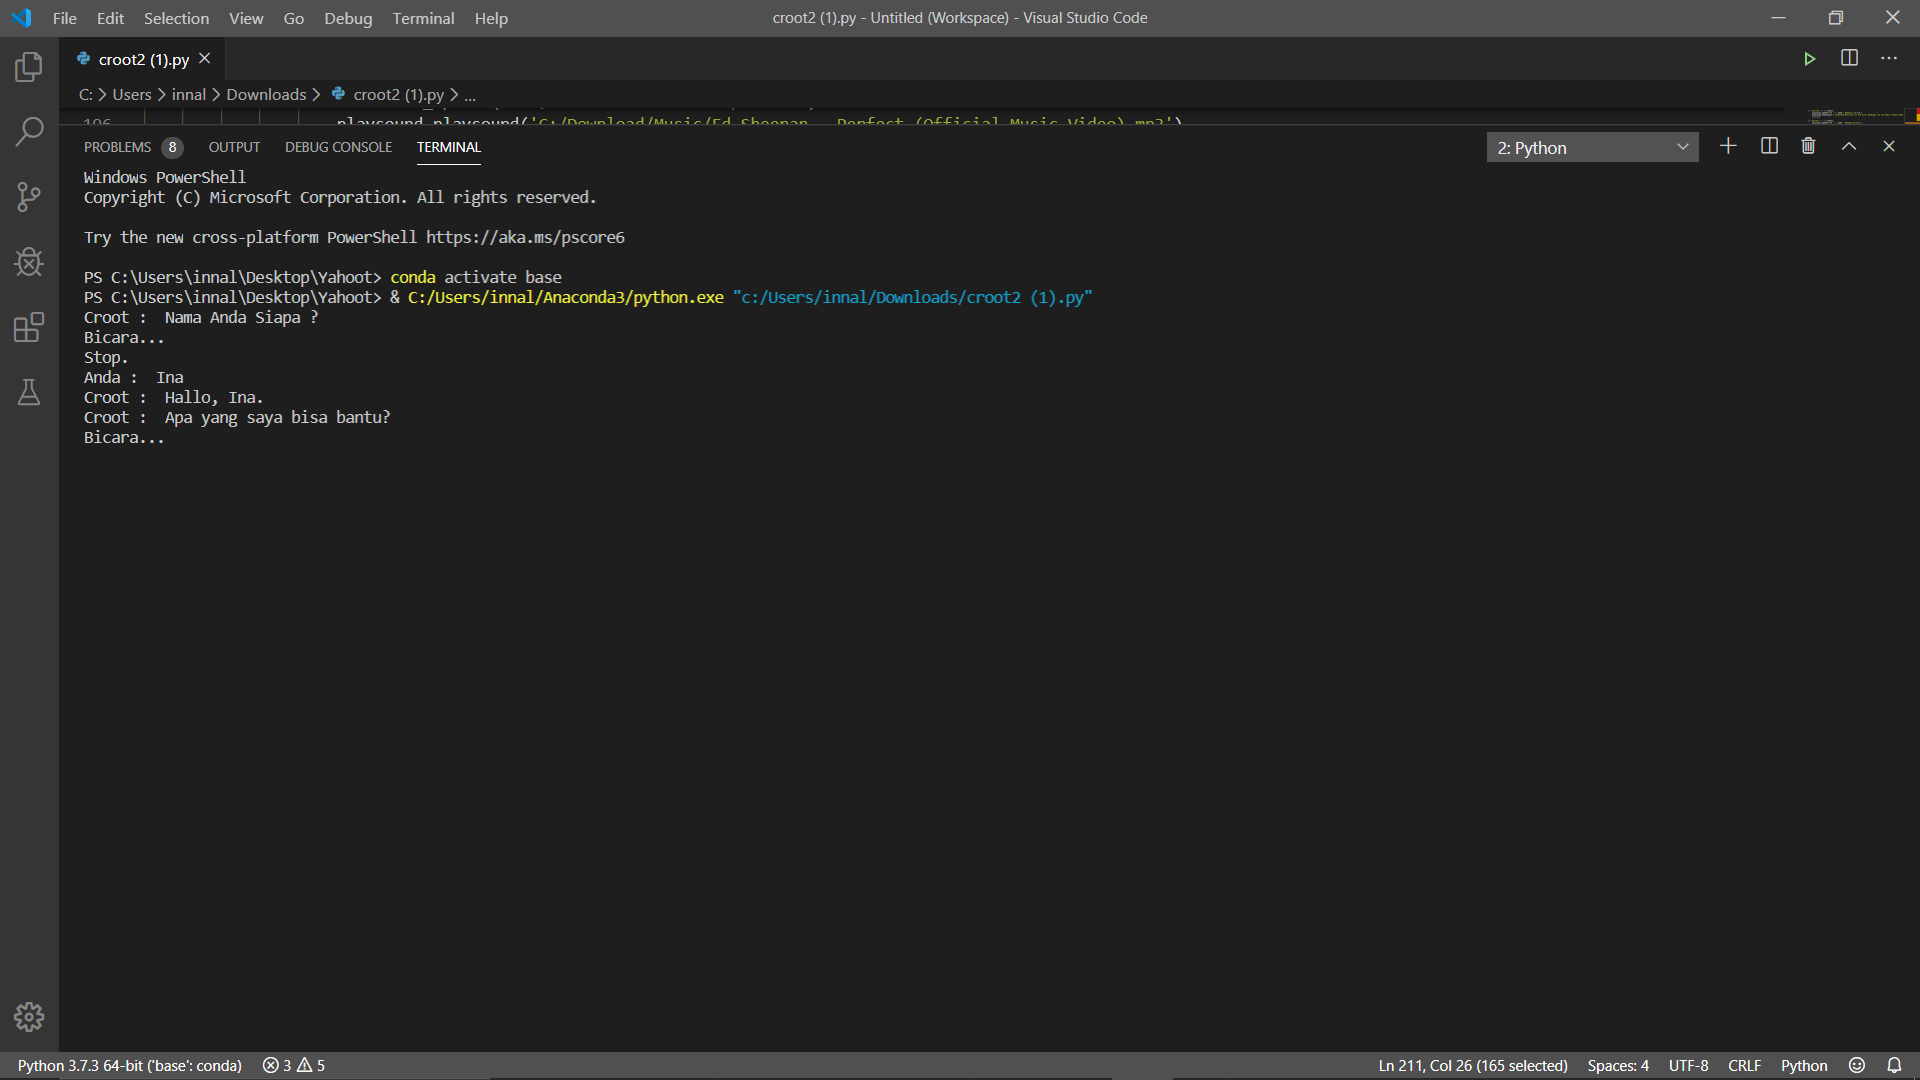
\includegraphics[width=1\textwidth]{tutorial selenium/figures/7q.png}
\caption{}
\label{}
\end{figure}
s
\\
\\
\\
\\
\\
s
\begin{figure}[H]
\centering
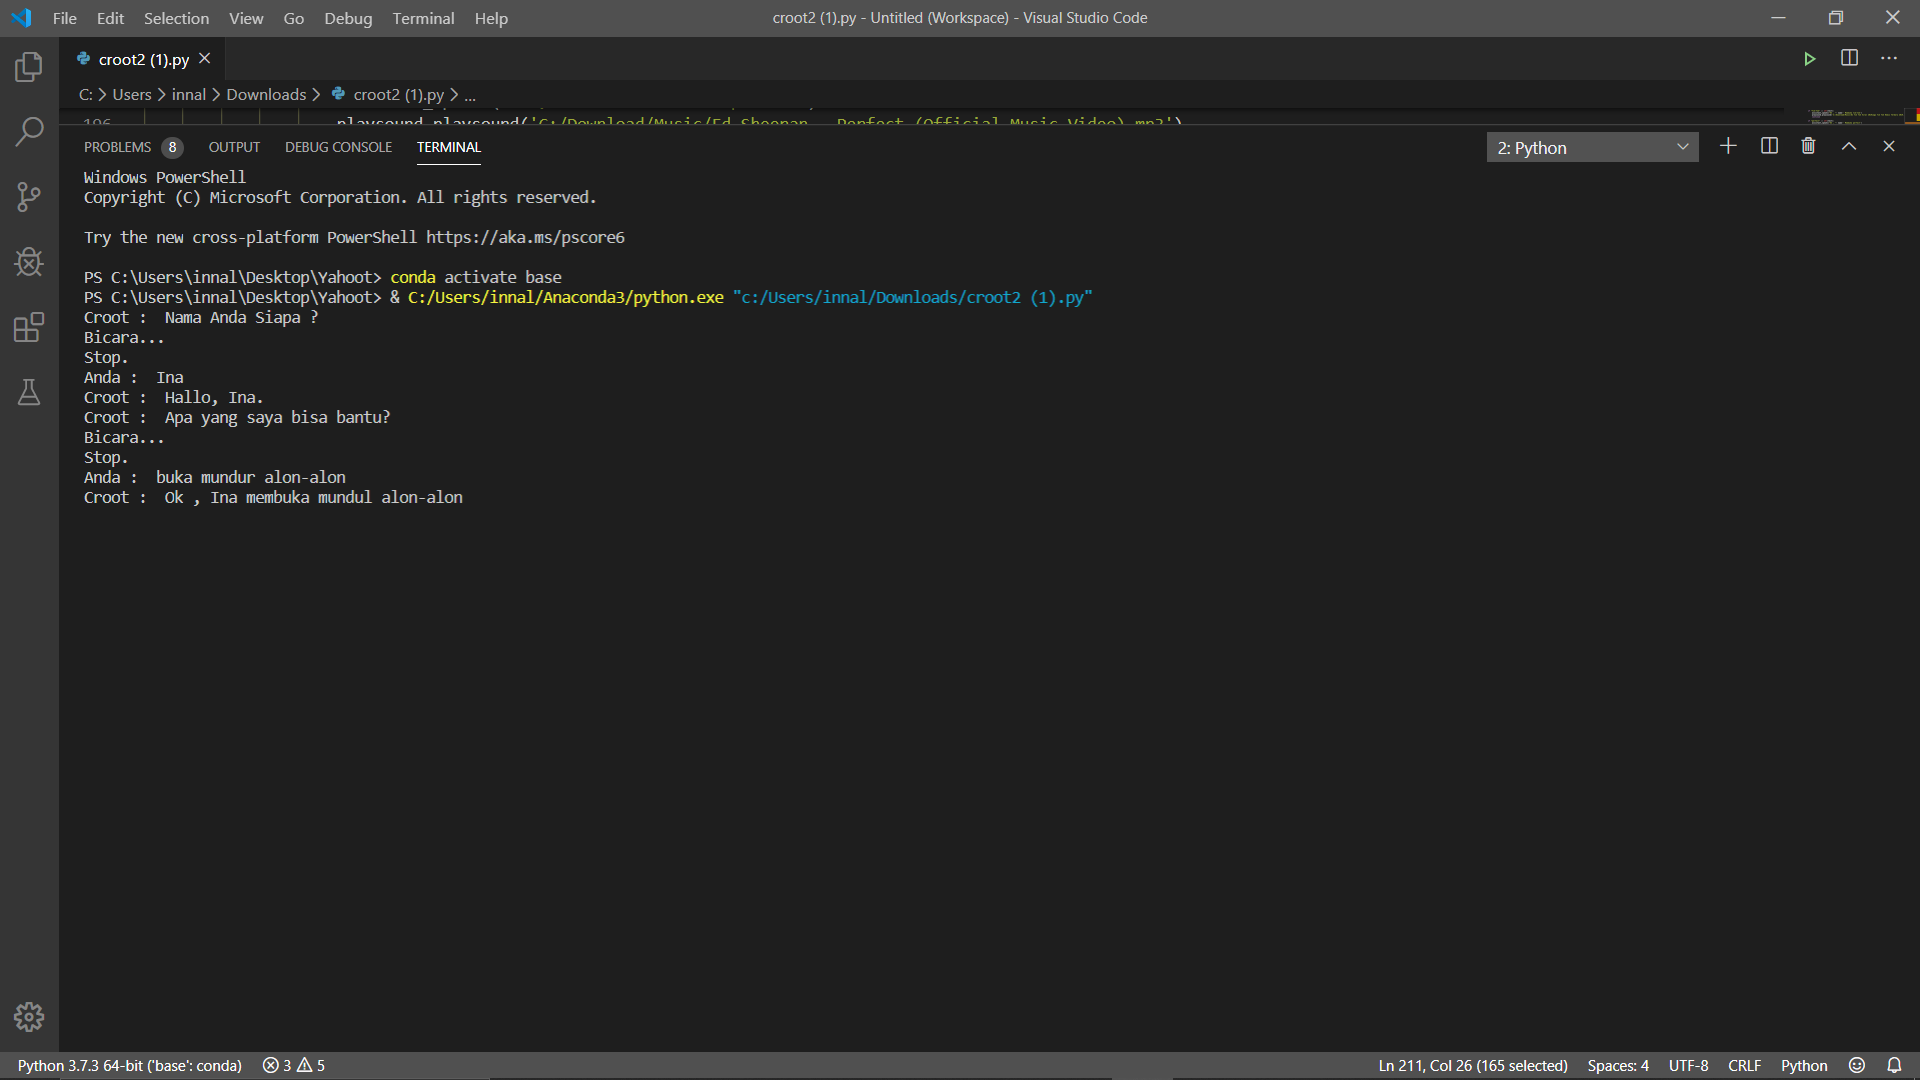
\includegraphics[width=1\textwidth]{tutorial selenium/figures/8q.png}
\caption{}
\label{}
\end{figure}
s
\\
\\
\\
\\
\\
\\
\\
s
\begin{figure}[H]
\centering
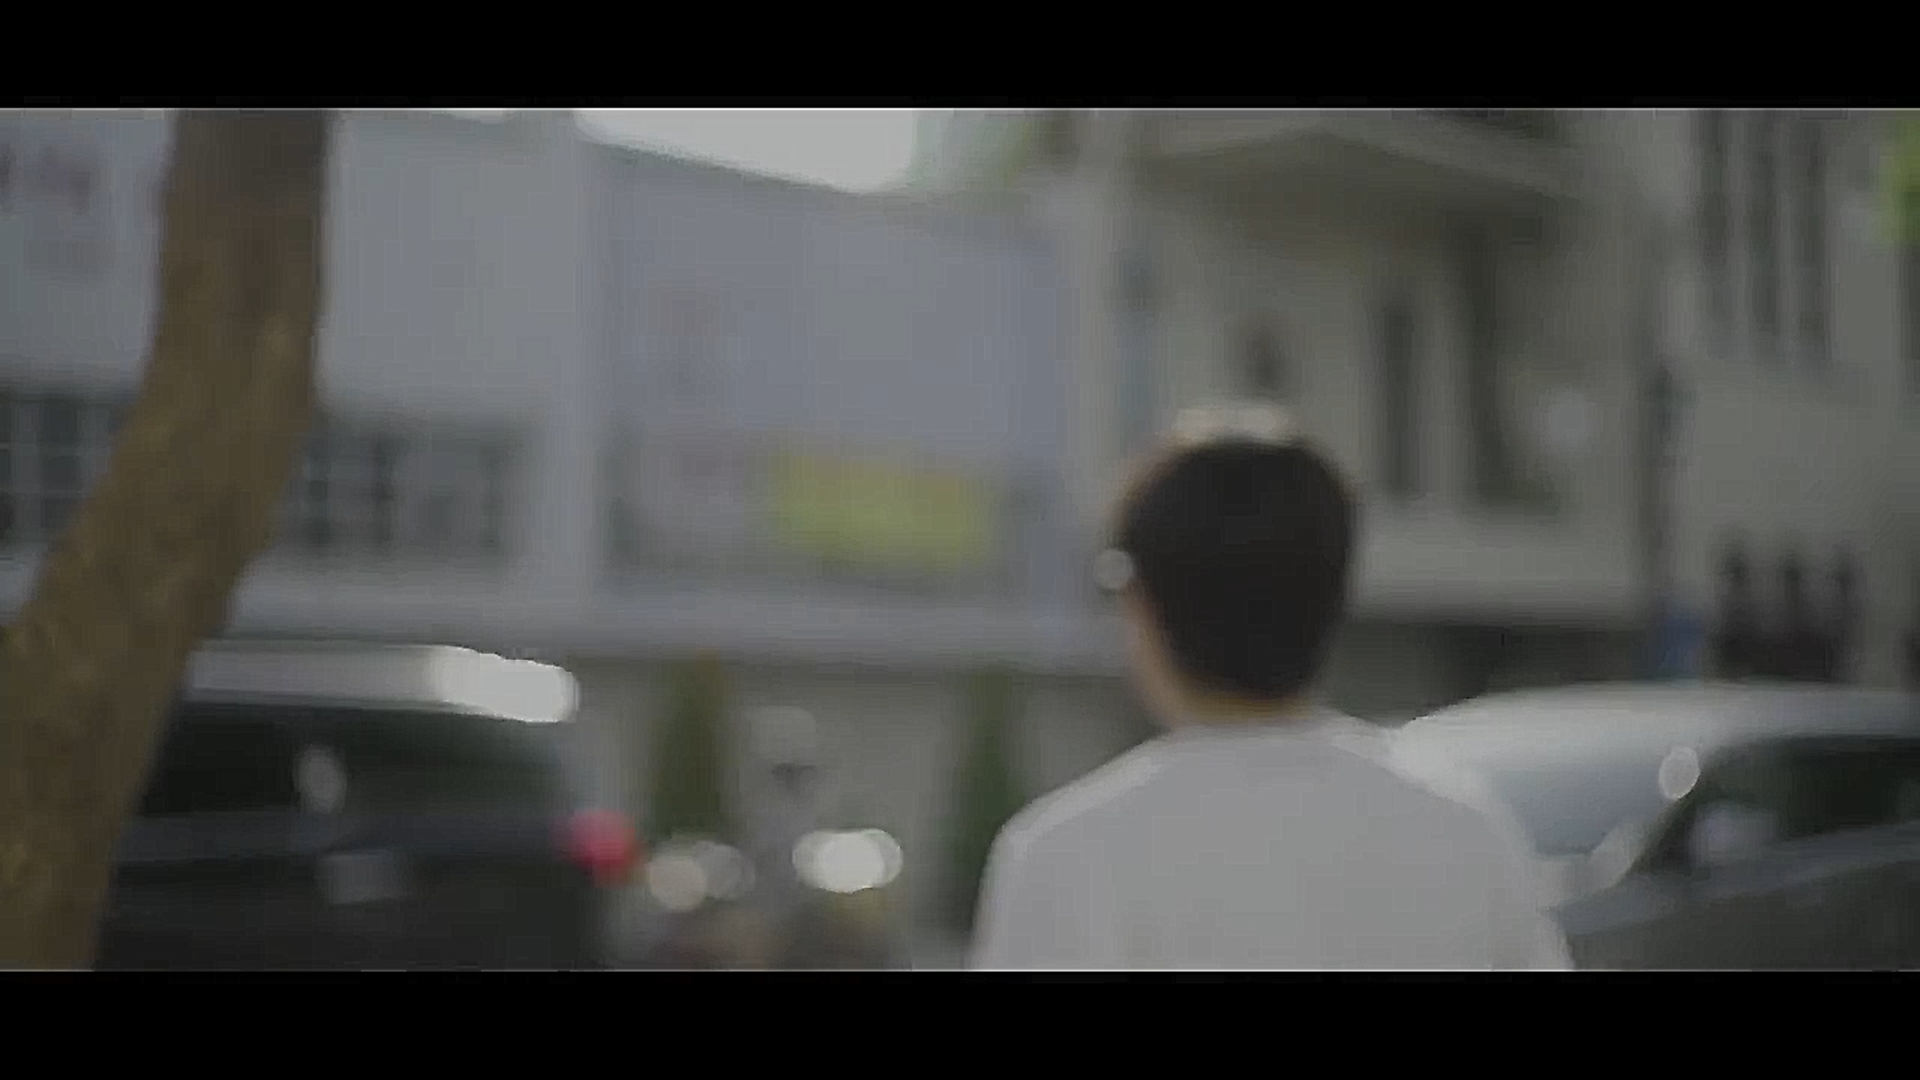
\includegraphics[width=1\textwidth]{tutorial selenium/figures/9q.png}
\caption{}
\label{}
\end{figure}
s
\\
\\
\\
\\
\\
\\
\\
\\
s
\begin{figure}[H]
\centering
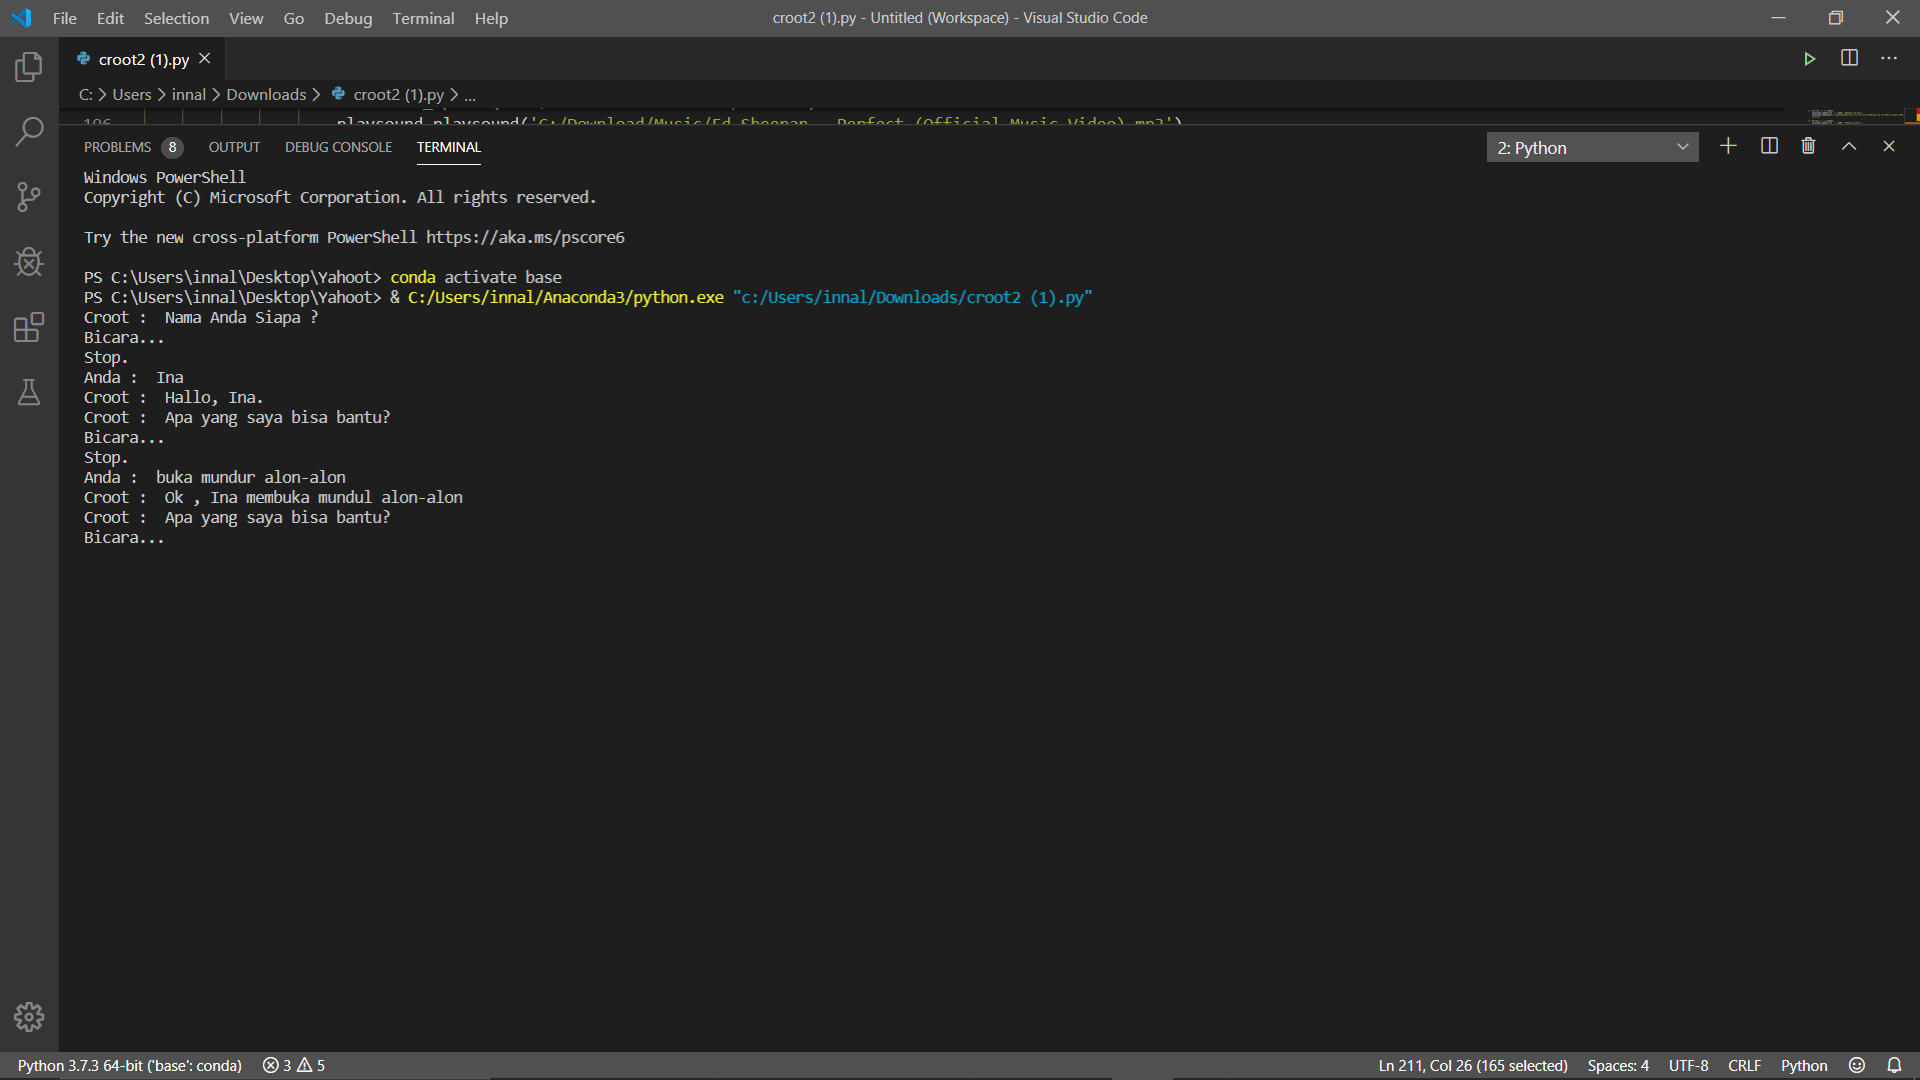
\includegraphics[width=1\textwidth]{tutorial selenium/figures/10q.png}
\caption{}
\label{}
\end{figure}
s
\\
\\
\\
\\
\\
\\
\\
\\
s
\begin{figure}[H]
\centering
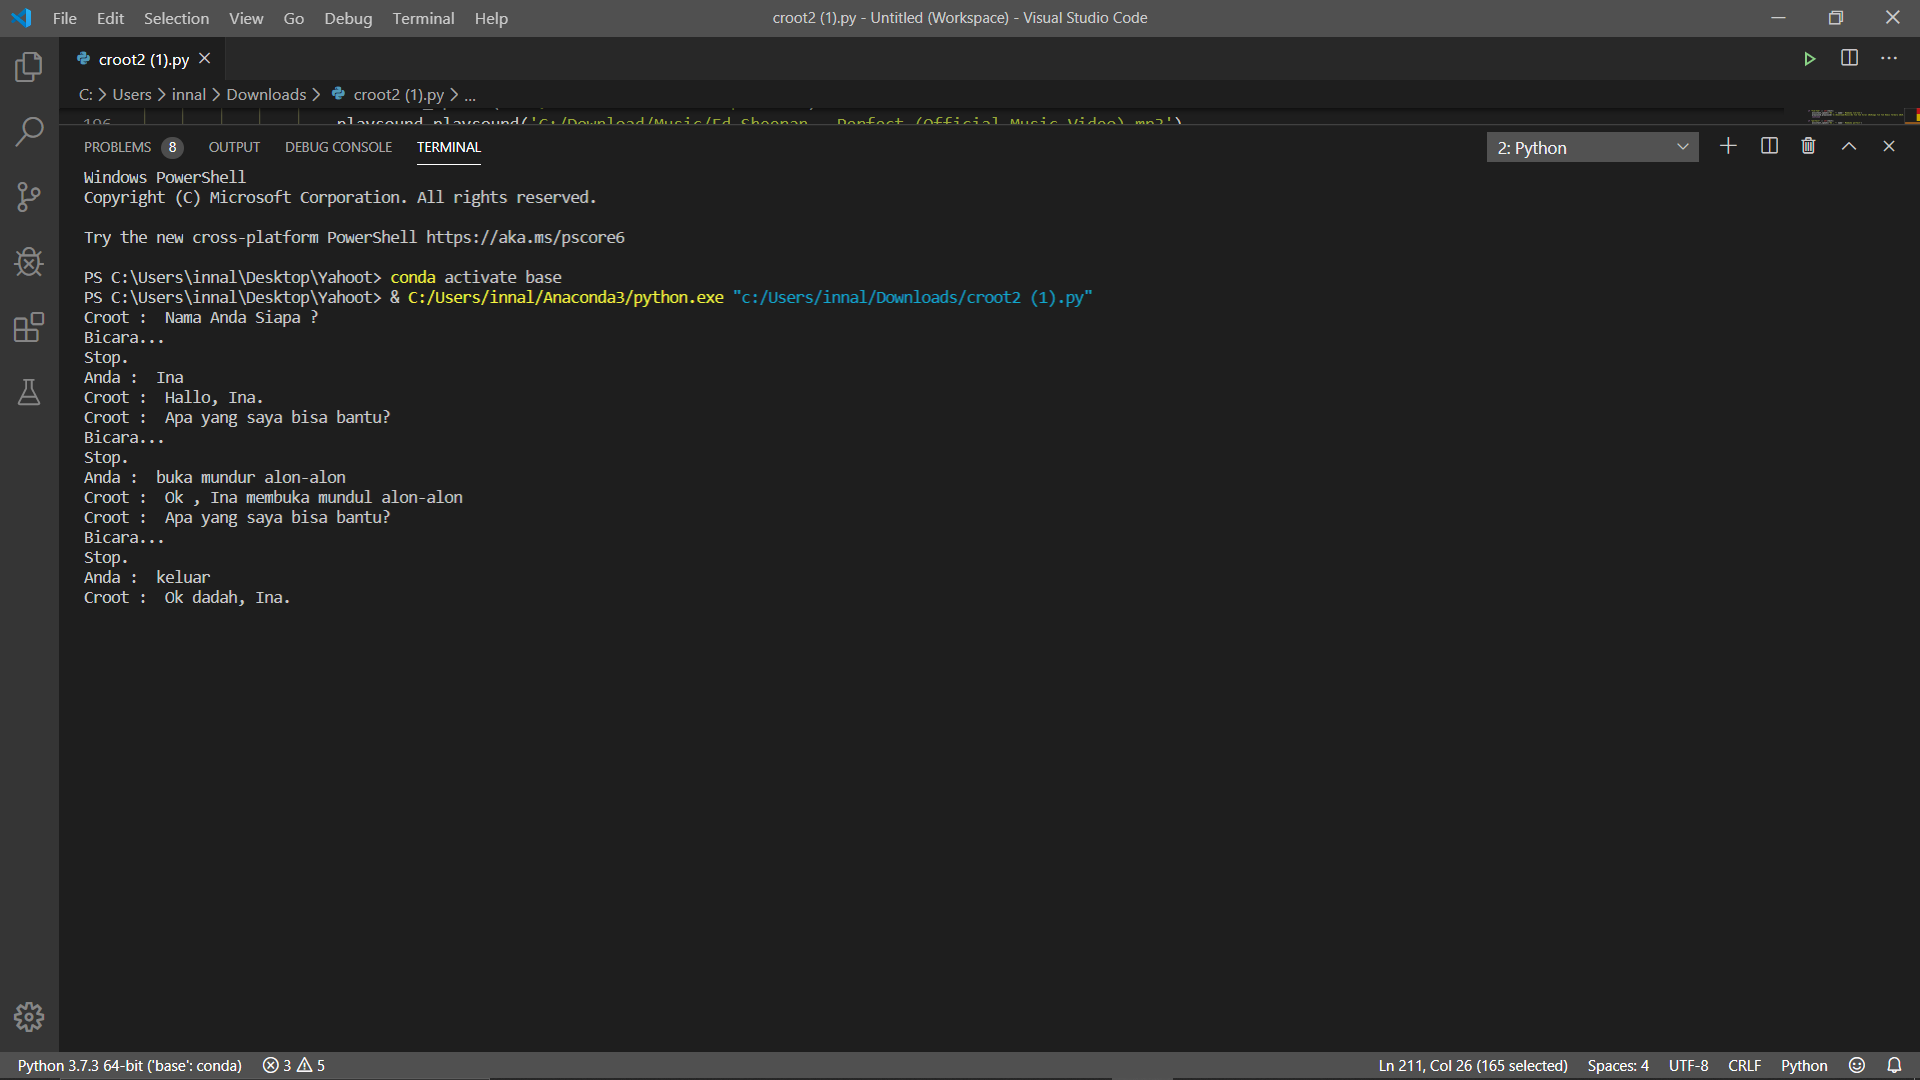
\includegraphics[width=1\textwidth]{tutorial selenium/figures/11q.png}
\caption{}
\label{}
\end{figure}
s
\\
\\
\\
\\
\\
\\
\\
\\
s
\begin{figure}[H]
\centering
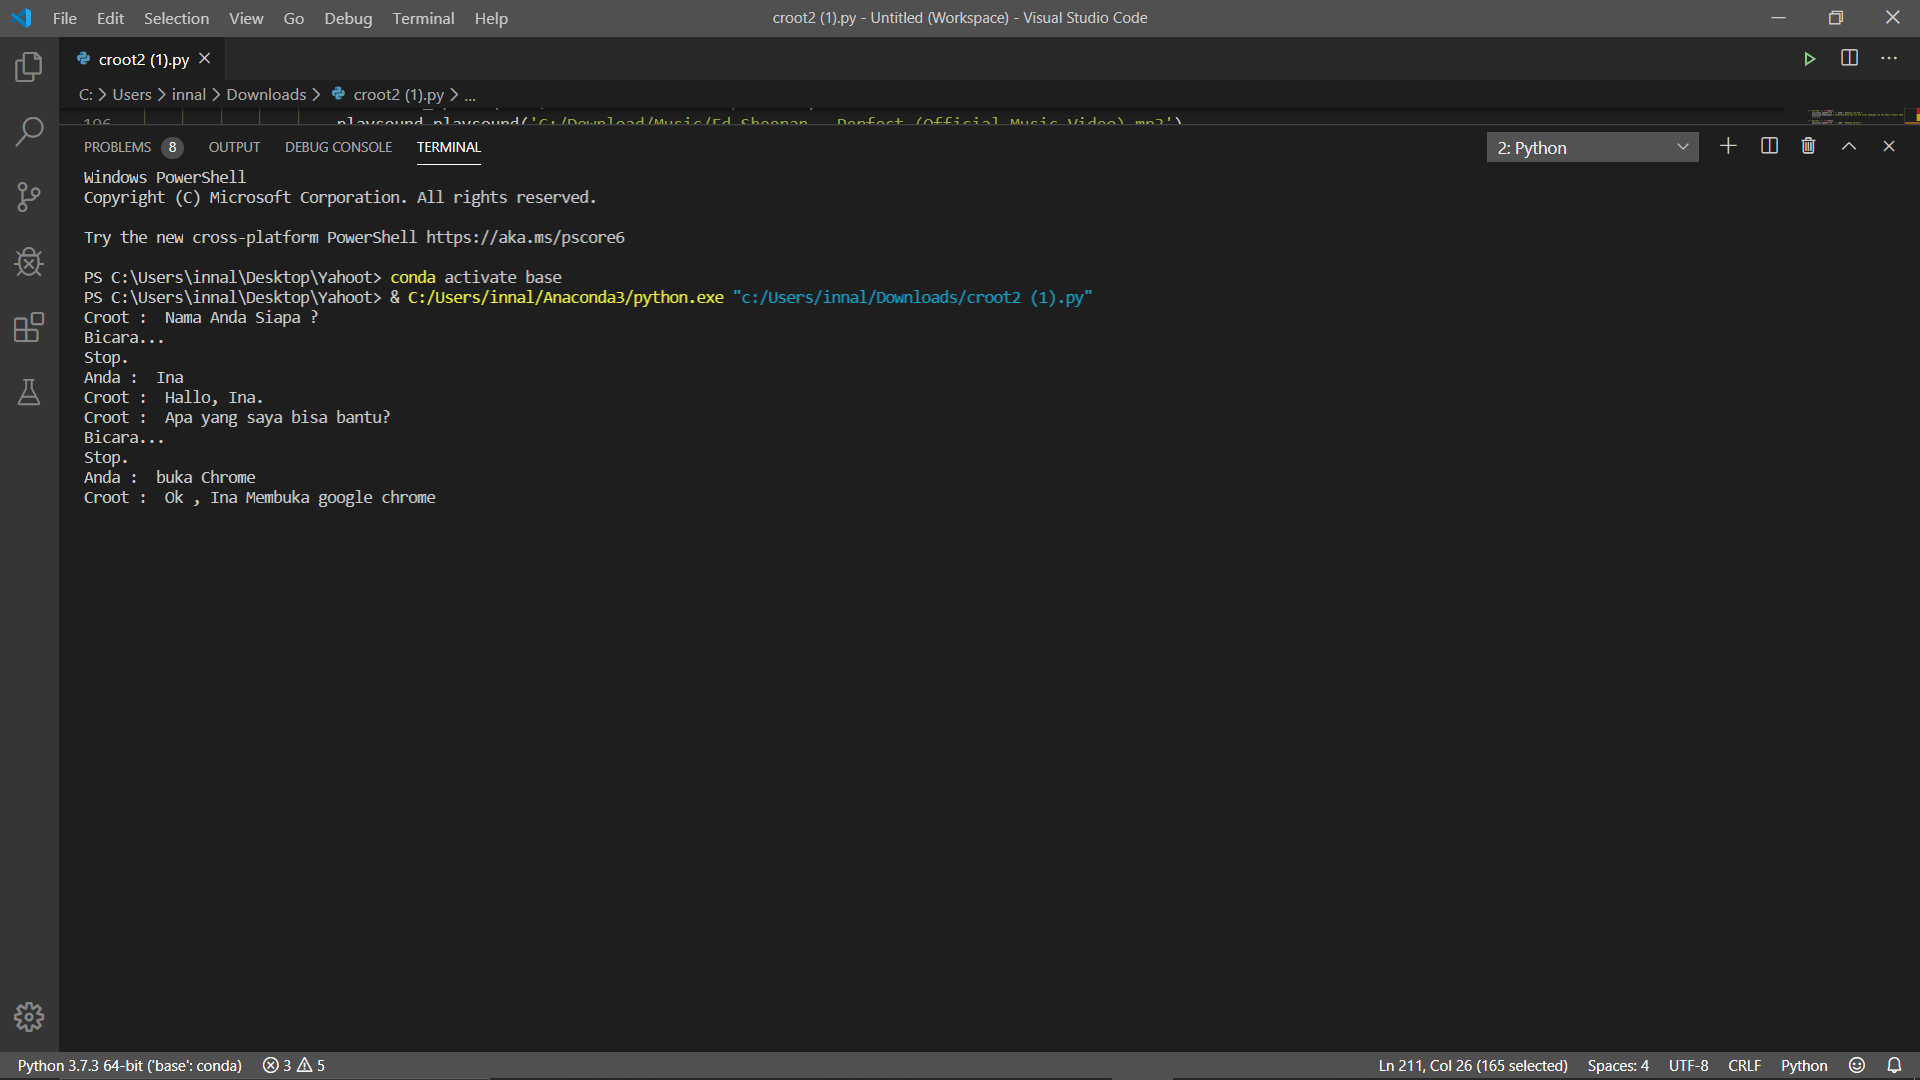
\includegraphics[width=1\textwidth]{tutorial selenium/figures/12q.png}
\caption{}
\label{}
\end{figure}
s
\\
\\
\\
\\
\\
\\
\\
\\
s
\begin{figure}[H]
\centering
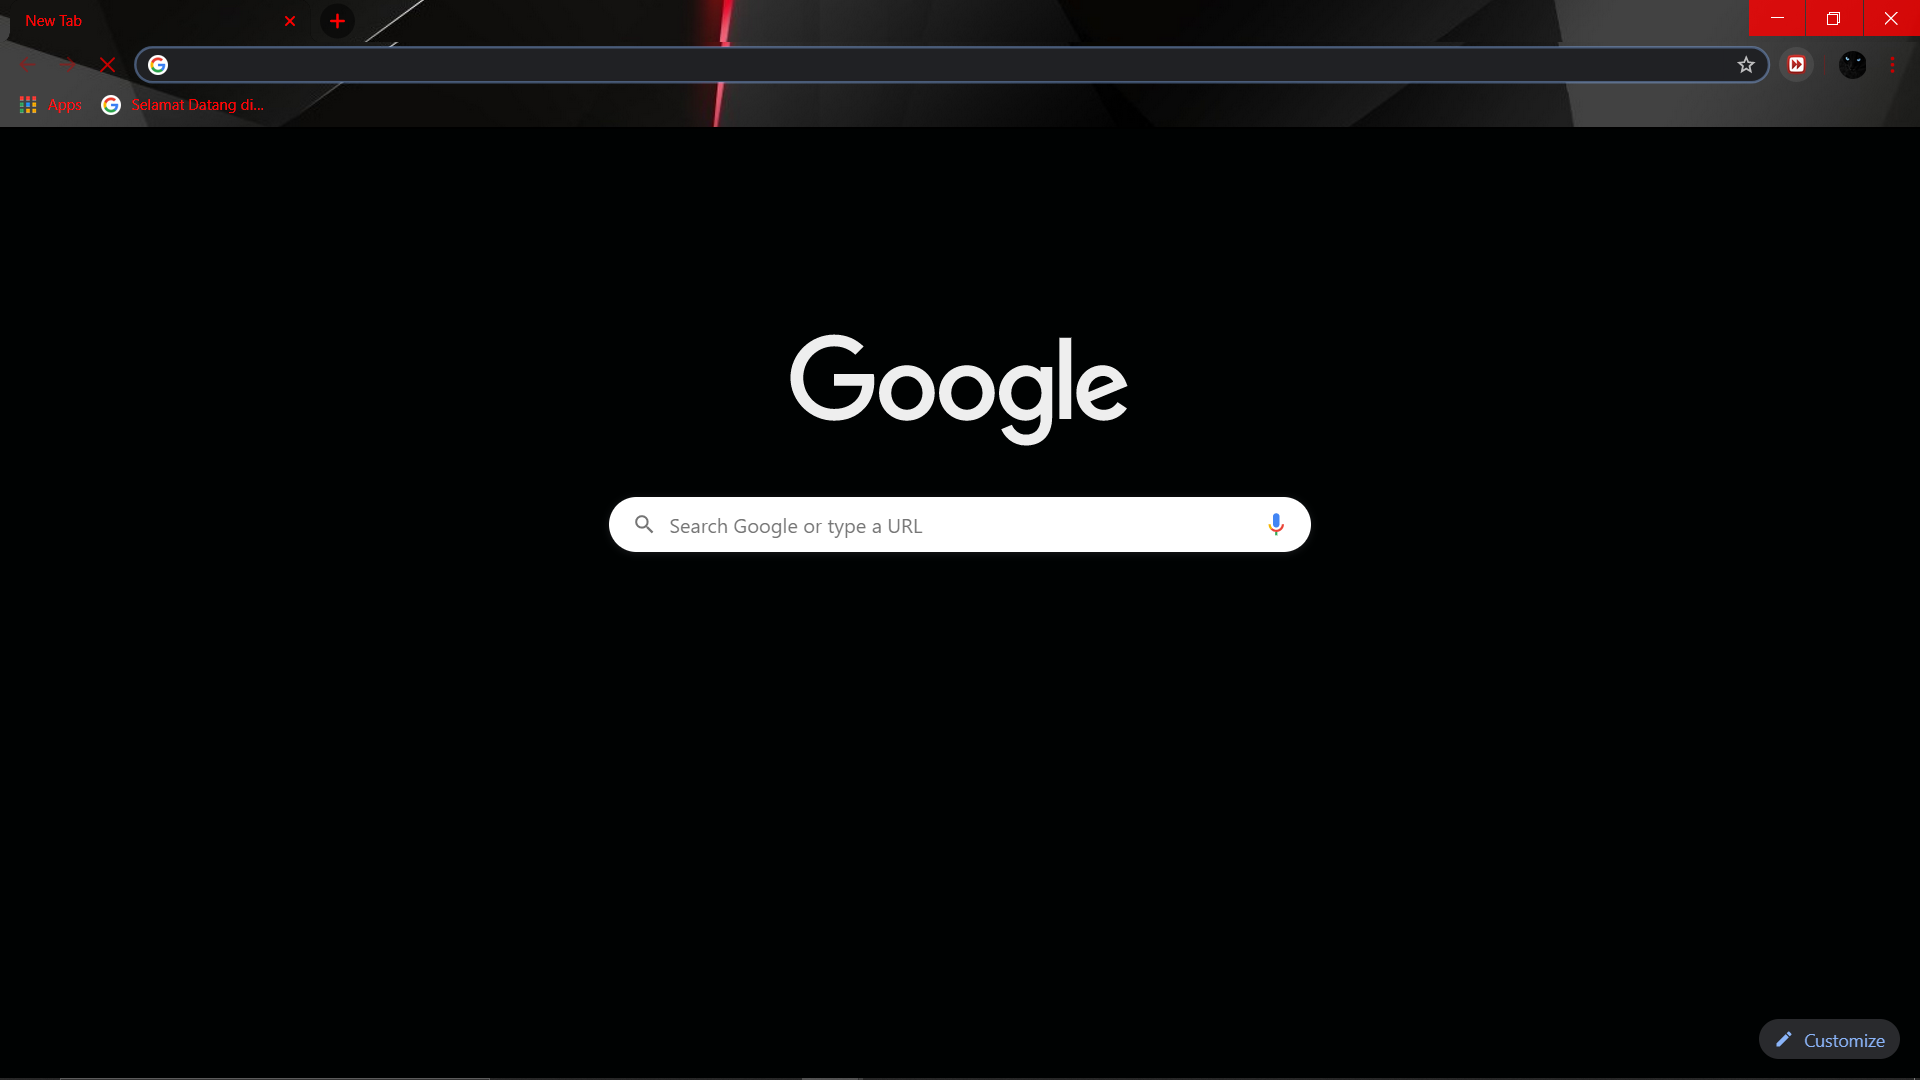
\includegraphics[width=1\textwidth]{tutorial selenium/figures/13q.png}
\caption{}
\label{}
\end{figure}
s
\\
\\
\\
\\
\\
\\
\\
\\
s
\begin{figure}[H]
\centering
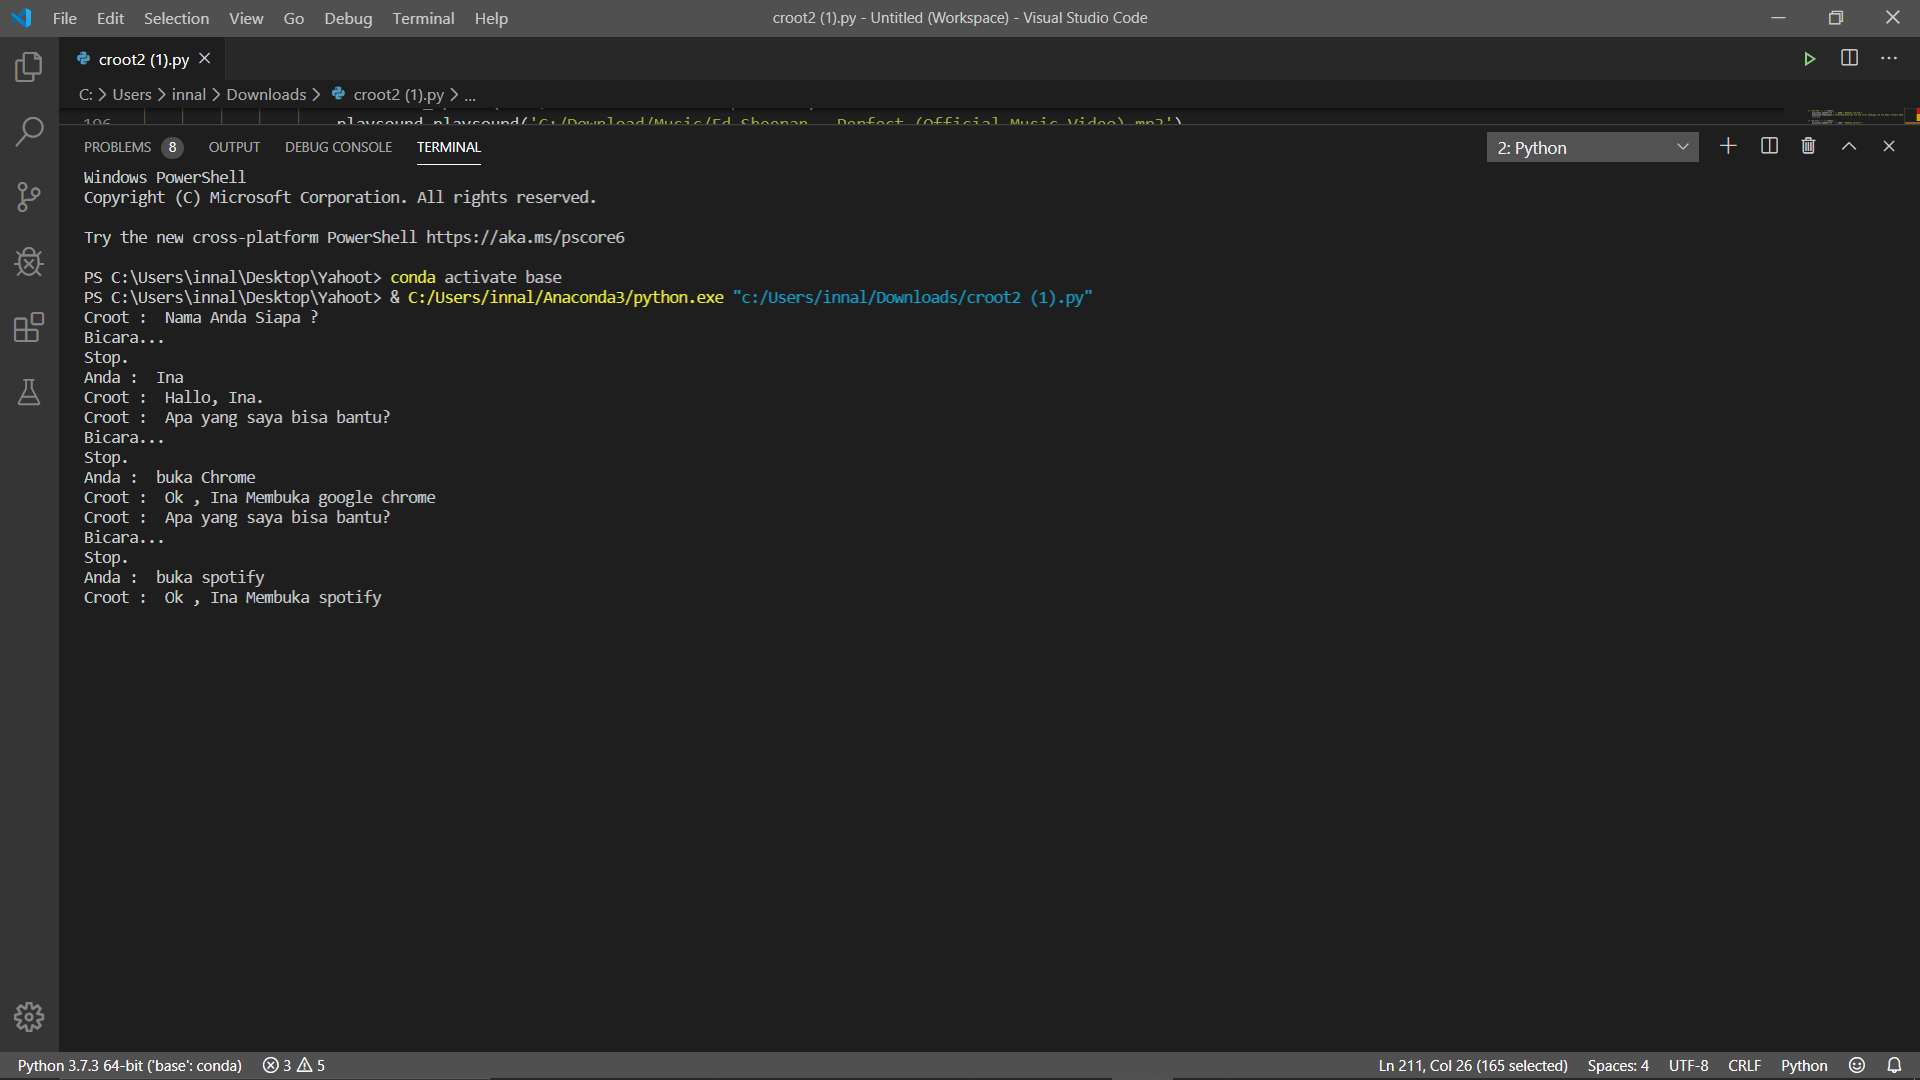
\includegraphics[width=1\textwidth]{tutorial selenium/figures/14q.png}
\caption{}
\label{}
\end{figure}
s
\\
\\
\\
\\
\\
\\
\\
\\
s
\begin{figure}[H]
\centering
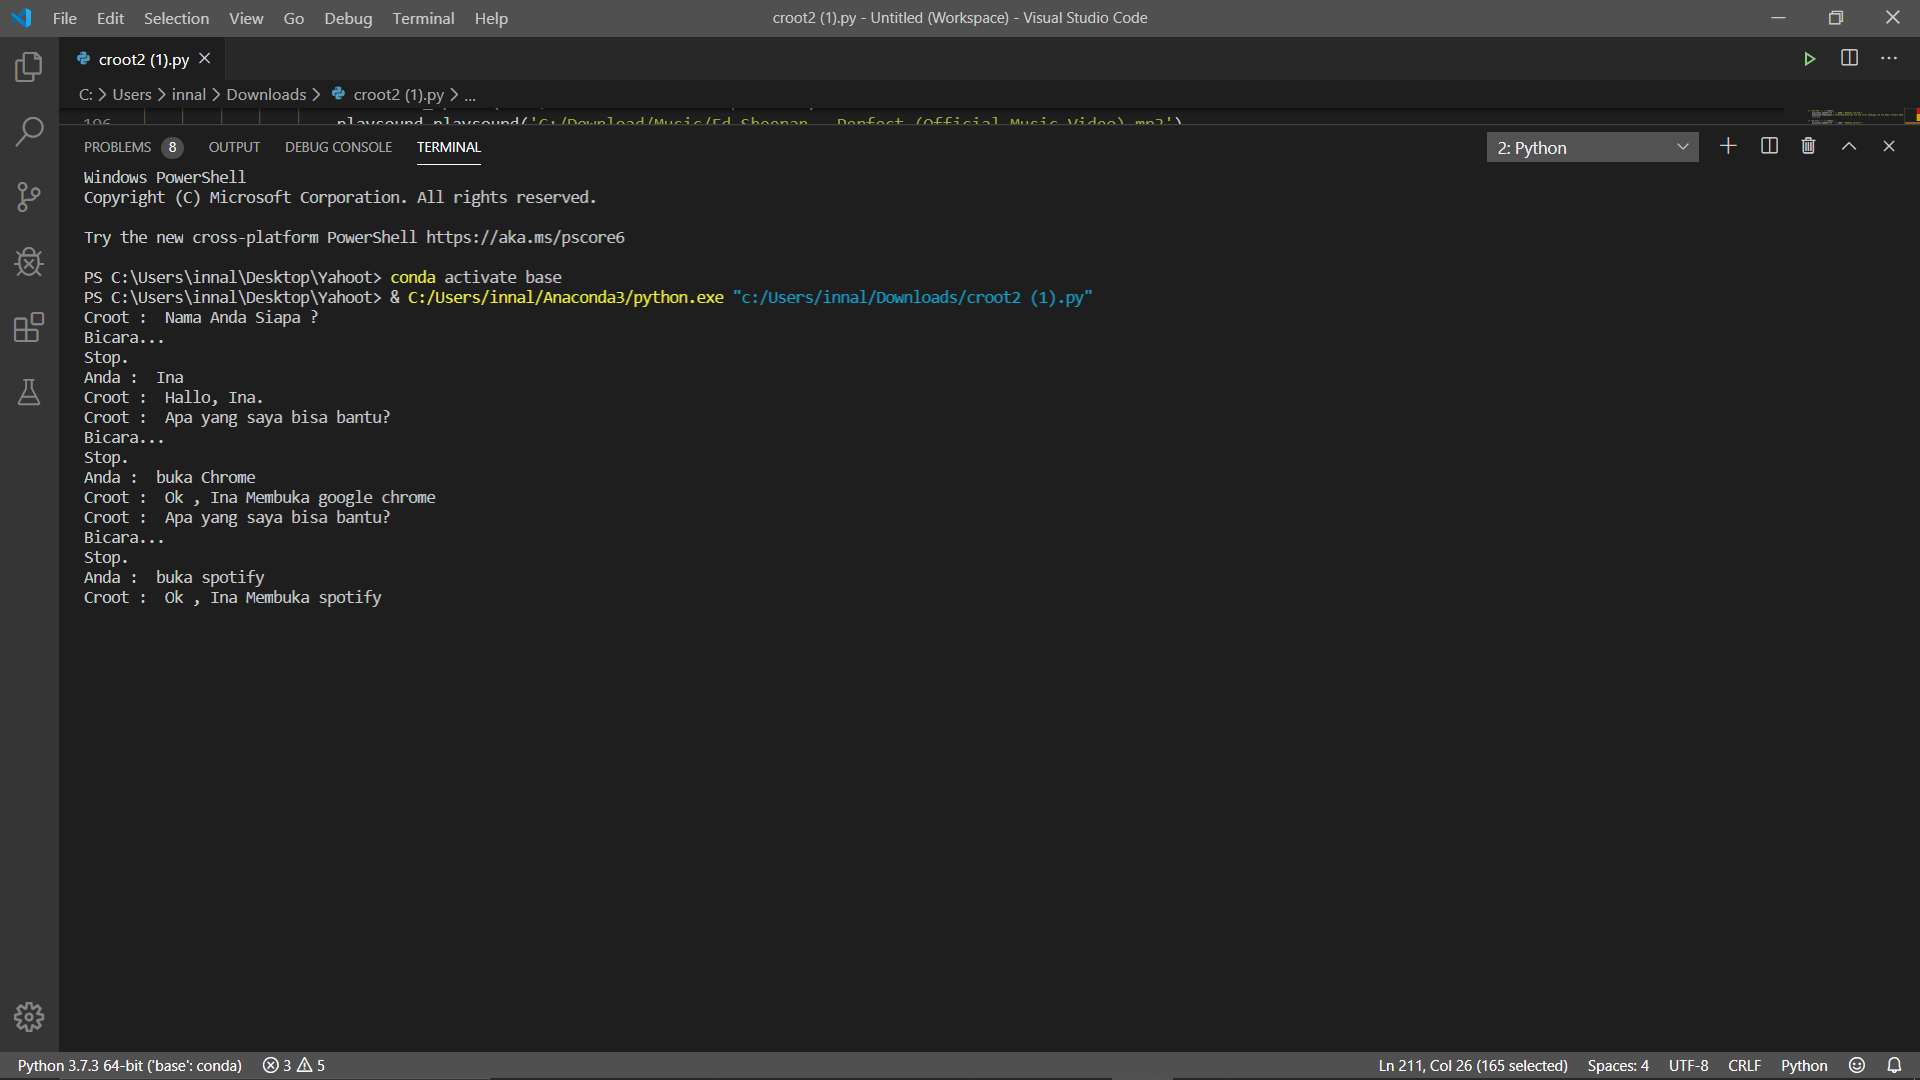
\includegraphics[width=1\textwidth]{tutorial selenium/figures/15q.png}
\caption{}
\label{}
\end{figure}
s
\\
\\
\\
\\
\\
\\
\\
\\
s
\begin{figure}[H]
\centering
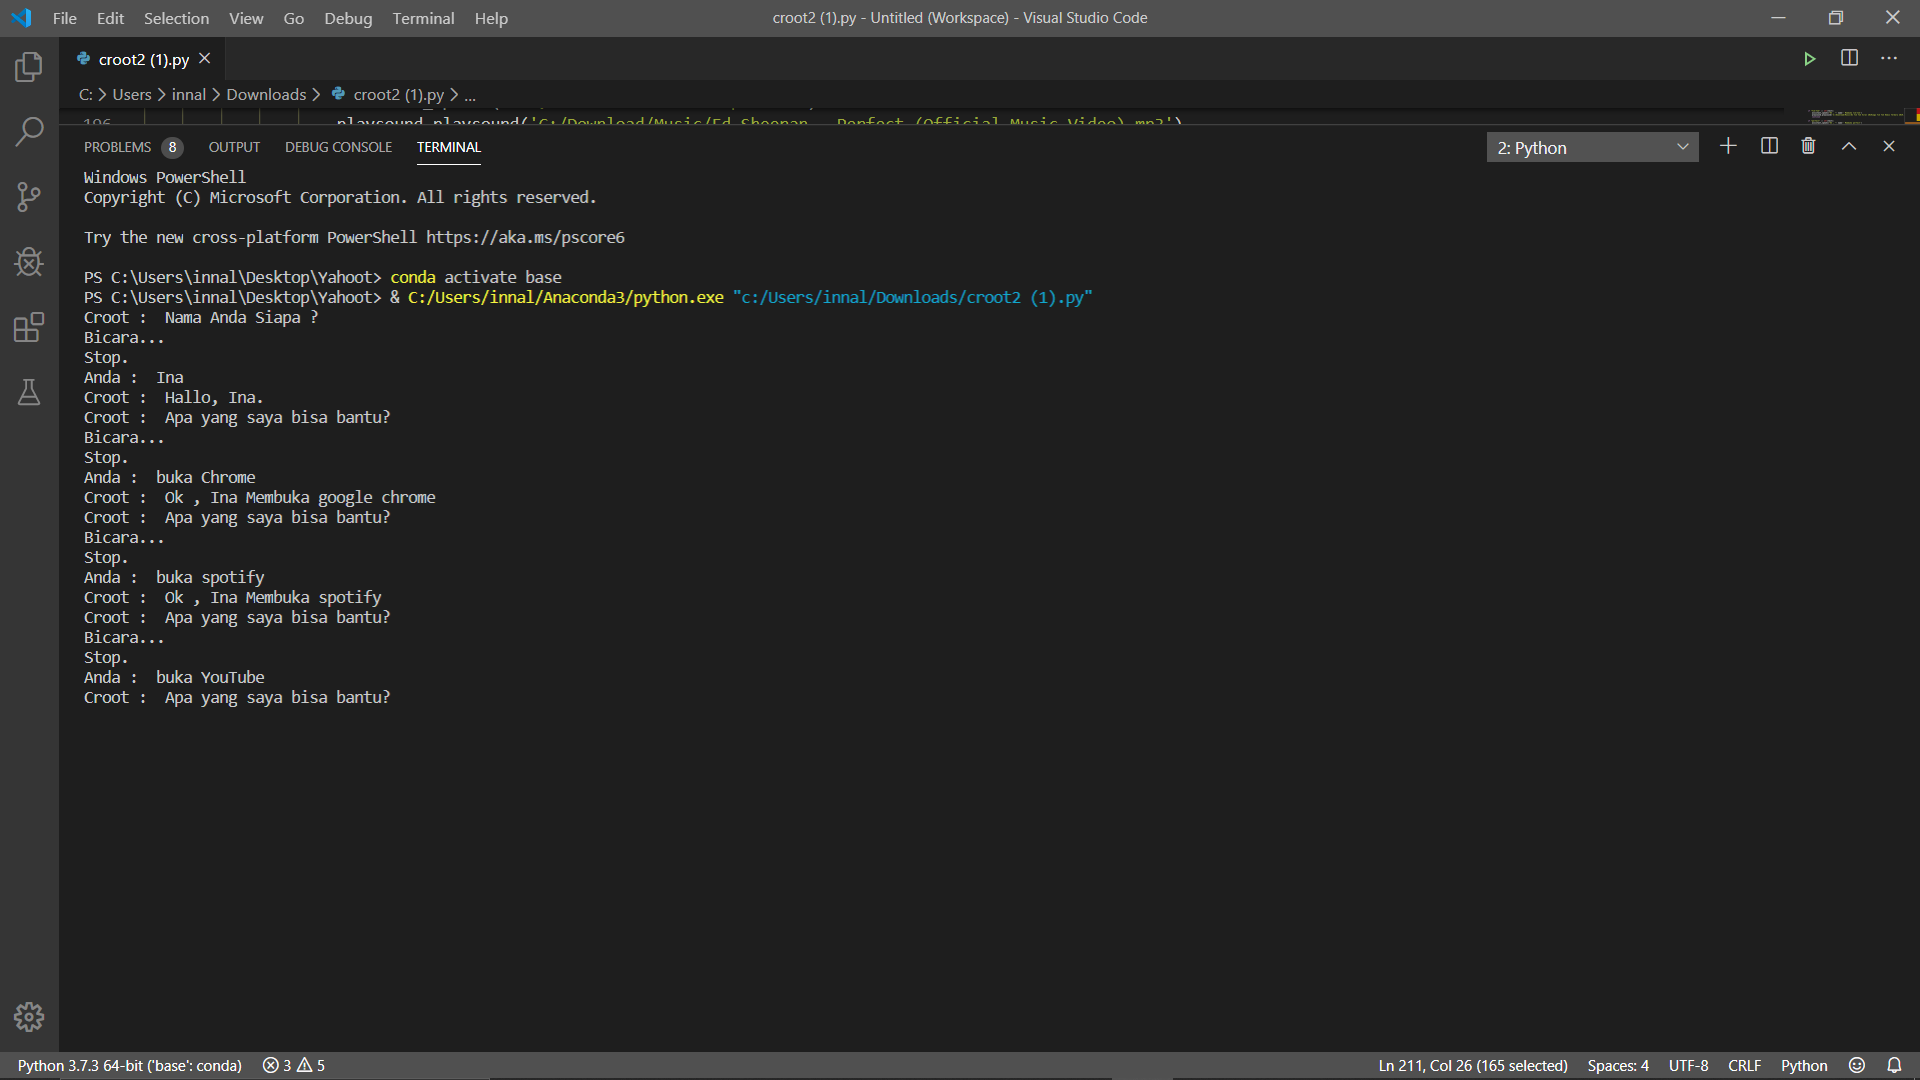
\includegraphics[width=1\textwidth]{tutorial selenium/figures/16q.png}
\caption{}
\label{}
\end{figure}
s
\\
\\
\\
\\
\\
\\
\\
\\
s
\begin{figure}[H]
\centering
\includegraphics[width=1\textwidth]{tutorial selenium/figures/17.png}
\caption{}
\label{}
\end{figure}
s
\\
\\
\\
\\
\\
\\
\\
\\
s
\begin{figure}[H]
\centering
\includegraphics[width=1\textwidth]{tutorial selenium/figures/18q.png}
\caption{}
\label{}
\end{figure}
s
\\
\\
\\
\\
\\
\\
\\
\\
s
\begin{figure}[H]
\centering
\includegraphics[width=1\textwidth]{tutorial selenium/figures/19q.png}
\caption{}
\label{}
\end{figure}
s
\\
\\
\\
\\
\\
\\
\\
\\
s
s
\\
\\
\\
\\
\\
\\
\\
\\
s
\begin{figure}[H]
\centering
\includegraphics[width=1\textwidth]{tutorial selenium/figures/20q.png}
\caption{}
\label{}
\end{figure}
s
\\
\\
\\
\\
\\
\\
\\
\\
s
\begin{figure}[H]
\centering
\includegraphics[width=1\textwidth]{tutorial selenium/figures/19q.png}
\caption{}
\label{}
\end{figure}
s
\\
\\
\\
\\
\\
\\
\\
\\
s
\begin{figure}[H]
\centering
\includegraphics[width=1\textwidth]{tutorial selenium/figures/19q.png}
\caption{}
\label{}
\end{figure}



\bibliographystyle{IEEEtran} 
%\def\bibfont{\normalsize}
\bibliography{references}


%%%%%%%%%%%%%%%
%%  The default LaTeX Index
%%  Don't need to add any commands before \begin{document}
\printindex

%%%% Making an index
%% 
%% 1. Make index entries, don't leave any spaces so that they
%% will be sorted correctly.
%% 
%% \index{term}
%% \index{term!subterm}
%% \index{term!subterm!subsubterm}
%% 
%% 2. Run LaTeX several times to produce <filename>.idx
%% 
%% 3. On command line, type  makeindx <filename> which
%% will produce <filename>.ind 
%% 
%% 4. Type \printindex to make the index appear in your book.
%% 
%% 5. If you would like to edit <filename>.ind 
%% you may do so. See docs.pdf for more information.
%% 
%%%%%%%%%%%%%%%%%%%%%%%%%%%%%%

%%%%%%%%%%%%%% Making Multiple Indices %%%%%%%%%%%%%%%%
%% 1. 
%% \usepackage{multind}
%% \makeindex{book}
%% \makeindex{authors}
%% \begin{document}
%% 
%% 2.
%% % add index terms to your book, ie,
%% \index{book}{A term to go to the topic index}
%% \index{authors}{Put this author in the author index}
%% 
%% \index{book}{Cows}
%% \index{book}{Cows!Jersey}
%% \index{book}{Cows!Jersey!Brown}
%% 
%% \index{author}{Douglas Adams}
%% \index{author}{Boethius}
%% \index{author}{Mark Twain}
%% 
%% 3. On command line type 
%% makeindex topic 
%% makeindex authors
%% 
%% 4.
%% this is a Wiley command to make the indices print:
%% \multiprintindex{book}{Topic index}
%% \multiprintindex{authors}{Author index}

\end{document}


